\documentclass[
  journal=pasa,
  manuscript=research-paper, %% or "review"
  year=2023,
  volume=37
]{cup-journal}

\usepackage{microtype,siunitx,booktabs}

\DeclareRobustCommand{\VAN}[3]{#2}
\let\VANthebibliography\thebibliography
\def\thebibliography{\DeclareRobustCommand{\VAN}[3]{##3}\VANthebibliography}

%%%%% AUTHORS - PLACE YOUR OWN PACKAGES HERE %%%%%
\usepackage{graphicx}	% Including figure files
\usepackage{amsmath}	% Advanced maths commands
\usepackage{amssymb}	% Extra maths symbols
\usepackage{xspace}
\usepackage{upgreek}
\usepackage{hyperref}

%%%%%%%%%%%%%%%%%%%%%%%%%%%%%%%%%%%%%%%%%%%%%%%%%%

%%%%% AUTHORS - PLACE YOUR OWN COMMANDS HERE %%%%%

% COMMANDS
\newcommand\ion[2]{\text{#1\,\textsc{\lowercase{#2}}}}	% ionization states

% COMMENTS
\newcommand{\SB}[1]{{\textcolor{purple}{#1}}}

% STELLAR LABELS
\newcommand{\Teff}{$T_\mathrm{eff}$\xspace}
\newcommand{\logg}{$\log g$\xspace}
\newcommand{\feh}{$\mathrm{[Fe/H]}$\xspace}
\newcommand{\numax}{$\nu_\mathrm{max}$\xspace}
\newcommand{\vmic}{$v_\mathrm{mic}$\xspace}
\newcommand{\vsini}{$v \sin i$\xspace}
\newcommand{\vrad}{$v_\mathrm{rad}$\xspace}

% NAMES
\newcommand{\TheCannon}{\textit{The Cannon}\xspace}
\newcommand{\sme}{\textsc{sme}\xspace}
\newcommand{\marcs}{\textsc{marcs}\xspace}
\newcommand{\Gaia}{\textit{Gaia}\xspace}
\newcommand{\TLF}{\Teff, \logg, and \feh}

% UNITS
\newcommand{\dex}{\,\mathrm{dex}}	% dex
\newcommand{\K}{\,\mathrm{K}}	% dex
\newcommand{\Msol}{\,\mathrm{M_\odot}} % Msol
\newcommand{\kpc}{\,\mathrm{kpc}}	% kpc
\newcommand{\mags}{\,\mathrm{mag}}	% mag
\newcommand{\yr}{\,\mathrm{yr}}	% Gyr
\newcommand{\Gyr}{\,\mathrm{Gyr}}	% Gyr
\newcommand{\eV}{\,\mathrm{eV}}	% eV
\newcommand{\Angstroem}{\,\text{\AA}}	% Angstroem
\newcommand{\kms}{\,\mathrm{km\,s^{-1}}}	% km/s
\newcommand{\kpckms}{\,\mathrm{kpc\,km\,s^{-1}}}	% kpc km/s
\newcommand{\kmkmss}{\,\mathrm{km^2\,s^{-2}}}	% km^2/s^2
\newcommand{\kmsMpc}{\,\mathrm{km\,s^{-1}\,Mpc^{-1}}}	% km/s/Mpc
\newcommand{\muHz}{\,\mathrm{\upmu Hz}} % micro Hz

\sisetup{detect-all,separate-uncertainty=true}

\title{The GALAH Survey: Data Release 4}

\author{S. Buder}
\affiliation{Research School of Astronomy \& Astrophysics, Australian National University, Canberra, ACT 2611, Australia}
\affiliation{ARC Centre of Excellence for All Sky Astrophysics in 3 Dimensions (ASTRO 3D), Australia}
\email[S. Buder]{sven.buder@anu.edu.au}

\author{Main contributors}
\author{survey builders}
\author{other co-authors with significant contribution}
\author{The GALAH Collaboration}
% \alsoaffiliation{Joint first authors}

%\handlingeditor{Excellent E Editor}

\doi{10.1017/pasa.2020.32}

\received {dd Mmm 2023}
\revised  {dd Mmm 2023}
\accepted {dd Mmm 2023}
\published{dd Mmm 2023}

\keywords{
Surveys; the Galaxy; methods: observational; methods: data analysis; stars: fundamental parameters; stars: abundances} %% First letter not capped
% \jel{Q11; Q12; D81; M31}
% \msc{Q14; Q18; E21}
% \abbreviations{
%     BDHS: Bangladesh Demographic and Health Survey, 
%     IDA: Fe-deficiency anaemia, 
%     IFA: Fe-folic acid, 
%     MNP: multiple micronutrient powder, 
%     VAD: vitamin A deficiency
% }

\begin{document}


%%%%%%%%%%%%%%%%%%%%%%%%%%%%%%%%%%%%%%%%%%%%%%%%%%%%%%%%%%%%%%%%%%%%%%%%%
\begin{abstract}
%%%%%%%%%%%%%%%%%%%%%%%%%%%%%%%%%%%%%%%%%%%%%%%%%%%%%%%%%%%%%%%%%%%%%%%%%

The stars in our Milky Way hold the chemical history of our Milky Way in their atmospheres as they wander through our Galaxy. Like bar codes, we can extract the chemical fingerprint of stars from high-resolution spectra. The fourth data release (DR4) of the Galactic Archaeology with HERMES (GALAH) Survey provides the chemical abundances of up to 31 elements for 827\,288 stars which have exquisite orbit information from the \Gaia satellite information.

For this data release, we utilise neural networks to simultaneously fit all stellar labels (stellar parameters and elemental abundances) for the full wavelength range. The neural networks are trained on grids of synthetic spectra that were computed with Spectroscopy Made Easy.

In a first iteration, we fit the best set of labels and in particular radial velocities for all 943\,654 spectra (including repeat observations). These are used to properly co-add spectra (for example of spectroscopic binaries without line-splitting) for the second major iteration. This loop uses the distances inferred from astrometric data of the \Gaia satellite and 2MASS photometry to self-consistently infer more accurate and precise surface gravities for each star.

Notable improvements of this data release are the newly available abundances of carbon and nitrogen from molecular features as well as the significantly improved precision and amount of elemental abundances, in particular for neutron-capture elements.

The combination of chemical compositions across multiple nucleosynthesis pats, orbit information, and age estimates for almost a million stars from GALAH DR4 provides a rich data set for Galactic exploration.

\end{abstract}

%%%%%%%%%%%%%%%%%%%%%%%%%%%%%%%%%%%%%%%%%%%%%%%%%%%%%%%%%%%%%%%%%%%%%%%%%
\section{INTRODUCTION AND WORKFLOW}
\label{sec:introduction}
%%%%%%%%%%%%%%%%%%%%%%%%%%%%%%%%%%%%%%%%%%%%%%%%%%%%%%%%%%%%%%%%%%%%%%%%%

\subsection{Motivation} \label{sec:motivation}

The history of our Milky Way galaxy is written in star light. By capturing and analysing this light of millions of stars, we can learn about the chemical composition of the material that was locked into stellar atmospheres billions of years ago and use stars as time capsules into the past evolution of the Milky Way. The light of stars can thus guide us to explore and map our environment, just as it has guided Aboriginal and Torres Strait Islander people on Country since tens of thousands of years.

With this fourth data release (DR4) from the Galactic Archaeology with HERMES (GALAH), we are proudly publishing the next set of measurements of stellar chemical abundances for almost a third of the elements of the elements of the periodic table that are created by stars. The initial motivation for measuring so many elemental abundances was laid out by \citet{DeSilva2015} and included the major motivation - chemical tagging - with the aim to trace back stars that were born together through their (expected) similar chemical compositions. The recent and ongoing efforts of GALAH and other surveys like the SDSS/APOGEE surveys \citep[e.g.][]{SDSSDR17, Kollmeier2017}, LAMOST \citep{Zhao2012}, \Gaia-ESO \citep{Gilmore2022}, or RAVE \citep{Steinmetz2020a} have taught us that the chemical evolution of our galaxy and stars is complex and we cannot (yet) recover stellar siblings due to limitations in our observations, analyses methods, and intrinsic changes to chemical composition due stellar evolution. New observations and innovations in the analysis that are presented in this data release, will allow us to make significant progress towards chemical tagging.

The unique observational setup of GALAH allows us to deliver the chemical information for a powerful and substantial set of stars: those which have exquisite orbit information from the revolutionary \Gaia satellite \citep{Gaia-Collaboration2016} and for which we can estimate stellar ages either from empirical or theoretical models, like stellar isochrones or mass- and age-dependent changes of chemical compositions. By combining stellar ages, orbits, and chemistry, we have made major advances in our understanding of our Galaxy. In particular, the discovery of the major merger of the Milky Way with another slightly less massive galaxy between 8 and $10\,\mathrm{Gyr}$ ago \citep{Belokurov2018, Helmi2018} was paradigm shifting and motivated a new rush to collect more and diverse information about the stars in our Milky Way.

The work of this data release is motivated by expanding the previous analysis of spectra towards a more holistic workflow that can aid upcoming surveys like 4MOST \citep{4MOST2019} and WEAVE \citep{Dalton2014}. Switching to the use of neural networks for interpolating synthetic spectra allows us to model the full wavelength range, molecular features such from $\mathrm{C_2}$ and CN molecules, rather then a small selection of wavelength windows around atomic lines. It even enables us to model all stellar labels (global parameters and elemental abundances) simultaneously and derive interstellar properties from the residuals of observations and synthetic stellar spectra. Finally, we can also relax the (often wrong) assumption that we observe single stars, by superimposing synthetic spectra of two stars, and thus provide global parameters for binary systems as part of our workflow.

\subsection{Workflow} \label{sec:workflow}

The workflow of GALAH DR4 is depicted in Fig.~\ref{fig:workflow_galah_dr4}. Following this workflow throughout this manuscript, we first describe the collection of data in Sec.~\ref{sec:data}, most notably the observation of HERMES spectra. We explain how we create synthetic stellar spectra to compare with the observed ones in Sec.~\ref{sec:synthetic_spectra}. The comparison is then done in two consecutive steps. In Sec.~\ref{sec:allspec_analysis}, we explain how we extract stellar labels from individual observations (without non-spectroscopic information folded in), while Sec.~\ref{sec:allstar_analysis} describes how we co-add repeated observations and fold in non-spectroscopic information for each star. Sec.~\ref{sec:binary_analysis} describes how we estimate main stellar labels for binary stars. We describe the post-processing of our data in Sec.~\ref{sec:post_processing} and validate our measurements in Sec.~\ref{sec:validation}. We describe the data products of this data release in Sec.~\ref{sec:catalogues_release_products} and conclude this manuscript in Sec.~\ref{sec:conclusion}.

\begin{figure}[hbt]
 \centering
 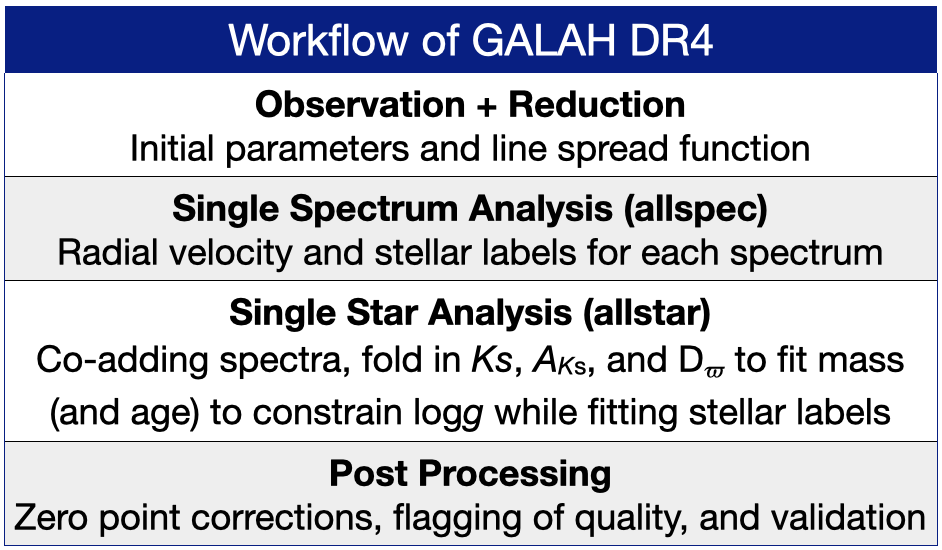
\includegraphics[width=\textwidth]{figures/workflow_galah_dr4.png}
 \caption{\textbf{Workflow of GALAH DR4}}
 \label{fig:workflow_galah_dr4}
\end{figure}

%%%%%%%%%%%%%%%%%%%%%%%%%%%%%%%%%%%%%%%%%%%%%%%%%%%%%%%%%%%%%%%%%%%%%%%%%
\section{DATA}
\label{sec:data}
%%%%%%%%%%%%%%%%%%%%%%%%%%%%%%%%%%%%%%%%%%%%%%%%%%%%%%%%%%%%%%%%%%%%%%%%%

The GALAH Survey is using the 3.9-metre Anglo-Australian Telescope at Siding Spring Observatory on Gamilaraay Country and its Two-Degree Field positioning system (2dF) topend \citep{Lewis2002}. 2dF places up to 400 fibre entrances on one of two plates which can be tumbled to allow parallel observing and fibre configuring. Light is then send through fibres to the High Efficiency and Resolution Multi-Element Spectrograph (HERMES) spectrograph \citep{Barden2010, Brzeski2011, Heijmans2012, Farrell2014, Sheinis2015} and dispersed into four non-contiguous wavelength bands in the optical and captured in separate rows of four separate charge-coupled devices (CCDs). The data used in this data release is primarily based on observations of stars with said setup, but also makes us of auxiliary photometric and astrometric information for the stars, where available.

In this Section, we describe which stars we have targeted and observed (Sec.~\ref{sec:target_selection_observations}) with the 2dF-HERMES setup, including the first description of the second phase of GALAH observations (GALAH Phase 2) with a sharper focus on main-sequence turnoff stars to estimate more precise ages. In Sec.~\ref{sec:spectroscopic_data_from_galah_observations}, we briefly summarise the properties of the spectroscopic data and how they were reduced to one-dimensional spectra. We also point out major changes of the observations and reductions with respect to the previous third data release \citep{Buder2021}. We further elaborate on the auxiliary information that was used for the analysis in Sec.~\ref{sec:non-spec_data}.

%%%%%%%%%%%%%%%%%%%%%%%%%%%%%%%%%%%%%%%%%%%%%%%%%%%%%%%%%%%%%%%%%%%%%%%%%
\subsection{Target selection and observational setup} \label{sec:target_selection_observations}
%%%%%%%%%%%%%%%%%%%%%%%%%%%%%%%%%%%%%%%%%%%%%%%%%%%%%%%%%%%%%%%%%%%%%%%%%

GALAH DR4 is a combination of the main GALAH survey and additional proposals to observe targets of the K2 \cite{Sharma2019} and TESS missions \cite{Sharma2018} to combine spectroscopic and asteroseismic data, as well as hand-picked and random observations of globular and open cluster members. The column \texttt{survey\_name} in our catalogues denotes this origin.

\subsubsection{Target selection of GALAH Phase 1 and 2}

For GALAH Phase 1, we used the 2MASS photometric survey \citep{Skrutskie2006} with its $J$ and $Ks$ filters as parent sample, from which we selected stars within empirical visual magnitudes
\begin{equation}
V_\mathrm{JK} = K_S+2(J-K_S+0.14)+0.382e^{((J-K_S-0.2)/0.5)}.
\end{equation}

For GALAH Phase 1, a tiling pattern (with unique \texttt{field\_id} entries) with $2\,\mathrm{deg}$ fields of view below declination $\delta < 10\,\mathrm{deg}$ were created for regions with Galactic latitude $\vert b \vert > 10\,\mathrm{deg}$ to avoid crowding and strong extinction. For each tile, a selection of 400 stars within magnitudes $9 < V_\mathrm{JK} < 12$ for a bright magnitude cut and $12 < V_\mathrm{JK} < 14$ for the nominal magnitude cut is randomly selected from the complete parent sample of 2MASS. This typically selects 2/3 main sequence and turnoff stars and 1/3 evolved stars.

For GALAH Phase 2, a stronger focus on turn-off stars was implemented with the photometric and astrometric information of \Gaia data release 2 as parent sample. For each field, we therefore first allocate fibres to stars with absolute magnitude between $2 < M_G < 4$, where
\begin{equation}
M_G = \texttt{phot\_g\_mean\_mag} + 5 \cdot \log_{10} \left( \frac{\texttt{parallax}}{100\,\mathrm{mas}} \right)
\end{equation}
with $G$ magnitude and parallax measurements from \Gaia DR2 \citep{Brown2018, Evans2018, Lindegren2018}. Remaining fibres are again filled with targets as done in Phase 1.

\subsubsection{Observational setup}

\begin{table}
\centering
 \caption{\textbf{Overview of stars observed for the programs included in this data release.} Numbers of open and globular cluster observations were estimated after observations as described in Sec.~\ref{sec:oc_gc}. We have observed 18 globular clusters (13 with $\geq$ 5 stars) and 286 open clusters (94 with $\geq$ 5 stars).}
\label{tab:field_ids}
\begin{tabular}{crcr}
\hline \hline
Program & Nr. Stars & Program & Nr. Stars \\
\hline
galah\_bright & 65\,188 & 
k2\_hermes & 117\,708\\
galah\_main & 427\,699 & 
tess\_hermes & 37\,228\\
galah\_faint & 25\,802 & 
globular clusters & 1\,185\\
galah\_phase2 & 125\,058 & 
open clusters & 4\,487\\
commissioning & 2\,625 & 
other & 20\,308\\
  \hline
 \end{tabular}
\end{table}

\begin{figure*}[ht]
 \centering
 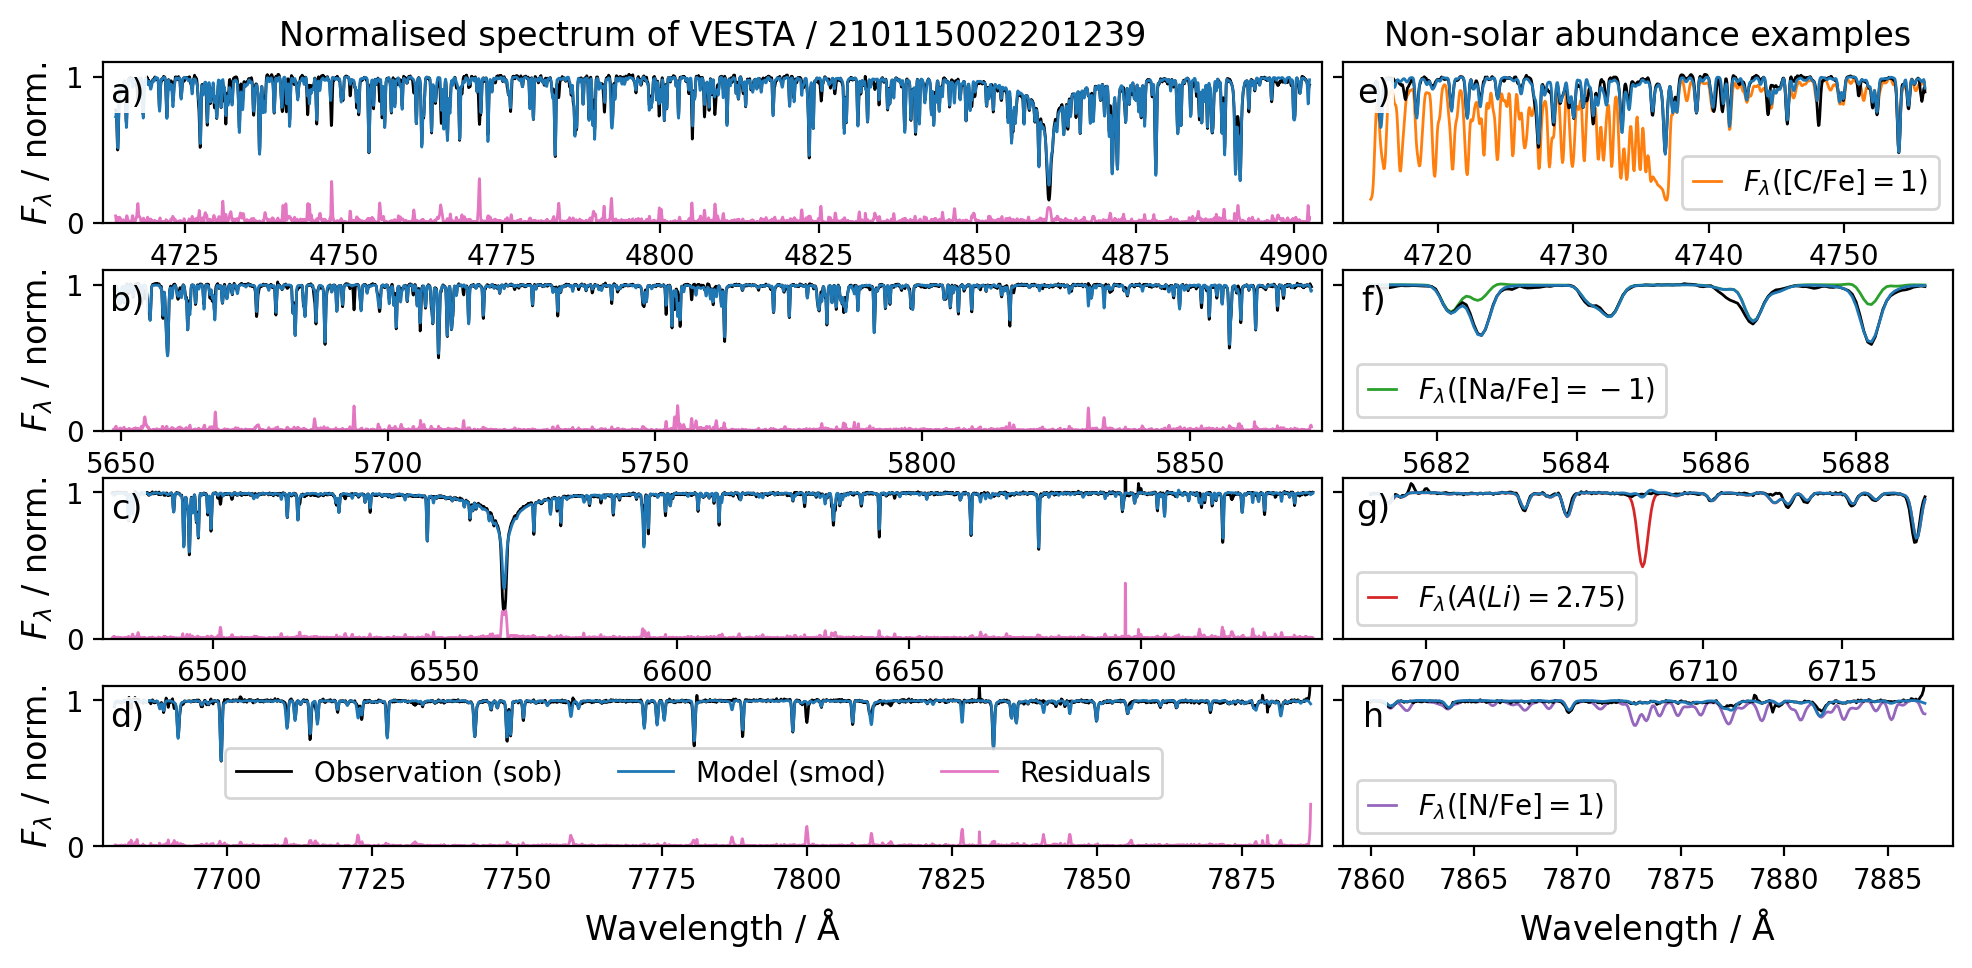
\includegraphics[width=\textwidth]{figures/210115002201239_abundance_examples.png}
 \caption{\textbf{Comparison of normalised observed (black) and synthetic spectra (blue) of the asteroid 4 Vesta with solar composition as well as examples of synthetic spectra with non-solar abundances.}
 \textbf{Panels a-d)} show the observed and best-fit synthetic spectrum as well as their absolute residual (pink) for the four wavelength channels of the HERMES spectrograph.
 \textbf{Panel e)} shows the beginning of the blue CCD 1 (left-most part of panel a) with an additional synthetic spectrum of ten-times higher C in orange, for which the $\mathrm{C}_2$ molecular absorption, the Swan bands, features would be prominent.
 \textbf{Panel f)} shows the beginning of the green CCD 2 (left-most part of panel b) and exemplifies with a synthetic spectrum in green that also a ten-times lower Na abundance (for example of accreted stars) can still be detected. 
 \textbf{Panel g)} shows the end of the red CCD 3 with a synthetic spectrum of primordial Li abundance of $\mathrm{A(Li)} = 2.75$ in red. While this abundance could be detected, the the line for the Solar value $\mathrm{A(Li)} = 1.05$ is barely detectable.
 \textbf{Panel h)} shows the end of the infrared CCD 4, which would show strong molecular absorption features of the CN molecule for $\mathrm{[N/Fe]} = 1$ (purple).
 }
 \label{fig:210115002201239_abundance_examples}
\end{figure*}

We list the observations under certain programs in Table~\ref{tab:field_ids}. Except for 2\,935 spectroscopic observations with the high-resolution mode of HERMES ($R \sim 42\,000$) on 7/8/10/11/$12^\text{th}$ February 2014, all observations were made in the low-resolution mode ($R \sim 28\,000$). Exposure times depend on programs. Under sufficient conditions (no clouds and seeing below $2\,\mathrm{arcsec}$), GALAH Phase 1 and TESS-HERMES observed 3x6 minutes for bright targets ($9 < V_\mathrm{JK} < 12$) and 3x20 minutes for the majority of targets ($12 < V_\mathrm{JK} < 14$). GALAH Phase 2 extended these times to 3x10 and 3x30 minutes, respectively, and included repeat observations of GALAH Phase 1 main targets with another 3x15 minutes. K2-HERMES observations targeted stars with $13 < V_\mathrm{JK} < 15$ or even $13 < V_\mathrm{JK} < 15.8$ to complement targets of the K2 Galactic Archaeology Program \citep{Stello2015} and were observed for 2 hours, similar to most globular and open cluster stars. Worse seeing conditions or thin clouds caused triggered between one ($2 < \mathrm{seeing} < 2.5\,\mathrm{arcsec}$) and 3 ($2.5 < \mathrm{seeing} < 3\,\mathrm{arcsec}$) additional exposures. In addition to the science frames, fibre flat and arc observations from a ThXe were taken before or after each exposure together with bias frames at the beginning of each night.

%%%%%%%%%%%%%%%%%%%%%%%%%%%%%%%%%%%%%%%%%%%%%%%%%%%%%%%%%%%%%%%%%%%%%%%%%
\subsection{Spectroscopic data from GALAH observations}
\label{sec:spectroscopic_data_from_galah_observations}
%%%%%%%%%%%%%%%%%%%%%%%%%%%%%%%%%%%%%%%%%%%%%%%%%%%%%%%%%%%%%%%%%%%%%%%%%

Since the commissioning of the HERMES spectrograph in late 2013 until 22 August 2022, the GALAH collaboration and its partners have observed and successfully reduced 943\,654 spectra of 827\,288 stars. The spectroscopic data is collected by four separate CCDs that cover $\sim 1000\,\text{\AA}$ in the range of $4713-4903$ (blue CCD or CCD1), $5648-5873$ (green / CCD2), $6478-6737$ (red / CCD3), and $7585-7887\,\text{\AA}$ (infrared IR / CCD4), as can be seen from the reduced example spectrum of the asteroid 4 Vesta in Fig.~\ref{fig:210115002201239_abundance_examples}. The reduction process to create FITS files of reduced spectra from two-dimensional images of the cameras is employing an updated and publicly available \href{https://github.com/sheliak/galah_reduction/blob/master/extract6.0.py}{version 6} of the already well-tested reduction pipeline \citep{Kos2017}. The extensions of these files are listed in Tab.~\ref{tab:reduction_fits} and created as follows.

\begin{table}
    \centering
    \caption{Data product 1: FITS files of reduced spectra}
    \label{tab:reduction_fits}
    \begin{tabular}{c|c}
    \hline \hline
    FITS Ext. & Description \\
    \hline
    Ext. 0 & Un-normalised signal~/~counts \\
    Ext. 1 & Normalised signal (by reduction pipeline) \\
    Ext. 2 & Relative uncertainty of signal \\
    Ext. 3 & Subtracted sky signal~/~counts \\
    Ext. 4 & Applied telluric correction \\
    Ext. 5 & Scattered light~/~counts \\
    Ext. 6 & Cross-talk \\
    Ext. 7 & Resolution profile~/~FWHM \\
    \hline
    \end{tabular}
\end{table}

Science frames are corrected by removing biases, fixing gains of the two CCD halfs, fixing bad pixels, dividing by master flats, as well as removing cosmics and scattered light. Subsequently, apertures are identified and use to extract the individual spectra. 

Wavelength calibrations are performed via Chebychev polynomial functions based on the ThXe arc frames and the spectra are interpolated onto a linearly increasing wavelength grid with starting wavelength \texttt{CRVAL1} and dispersion \texttt{CDELT1}. Both values are saved in the headers of the FITS files.

Finally, sky lines are subtracted and telluric lines removed, before a barycentric correction is applied to create the 'reduced' spectra that are saved in extension 1 of the reduction pipeline FITS files and used for the subsequent analysis. 

Noise / uncertainties are saved in extension 2 and calculated from the square root of the sum of flux, sky features (extension 3)\footnote{\SB{telluric features (extension 4) are not added in line 3424 of extract6.0.py.}}, scattered light (extension 5), crosstalk (extension 6) and as well as the squared readout noise.

The wavelength dependent line spread functions (LSFs) are measured from the arc calibration frames for each spectrum and CCD by fitting modified Gaussian distributions with a boxiness parameter $b$ and full width half maxima $fwhm$ for each wavelength point of the spectrum, that is
\begin{align}
    \exp \left(-0.693147 \vert 2 \cdot \textbf{\textit{x}}/\texttt{fwhm}\vert^\texttt{b}\right) \label{eq:lsf}
\end{align}
The array $\textbf{\textit{x}}$ then includes the pixels around each wavelength step that are used to apply the convolution from higher resolution to GALAH resolution spectra. The fitted values of $fwhm$ are saved in extension 7 with $b$ in its header.

\SB{Should we elaborate on any overall information, like SNR overview and pointing on the sky?}
\SB{Elaborate on how the reduction pipeline parameters \texttt{teff\_r} etc. are estimated.}

%%%%%%%%%%%%%%%%%%%%%%%%%%%%%%%%%%%%%%%%%%%%%%%%%%%%%%%%%%%%%%%%%%%%%%%%%
\subsection{Auxiliary data from \Gaia, 2MASS, and literature} \label{sec:non-spec_data}
%%%%%%%%%%%%%%%%%%%%%%%%%%%%%%%%%%%%%%%%%%%%%%%%%%%%%%%%%%%%%%%%%%%%%%%%%

%SELECT
%galah.sobject_id,
%tmass.designation as tmass_id,
%tmass.ph_qual as tmass_ph_qual,
%tmass.ra as raj2000,
%tmass.dec as dej2000,
%tmass.j_m, tmass.j_msigcom,
%tmass.h_m, tmass.h_msigcom,
%tmass.ks_m, tmass.ks_msigcom,
%calj.r_med_geo,calj.r_lo_geo,calj.r_hi_geo,
%calj.r_med_photogeo,calj.r_lo_photogeo,calj.r_hi_photogeo,
%calj.flag as calj_flag,
%gaia.*
%FROM gaiadr3.gaia_source as gaia
%LEFT OUTER JOIN
%	external.gaiaedr3_distance as calj
%	ON calj.source_id = gaia.source_id
%LEFT OUTER JOIN
%	gaiadr3.tmass_psc_xsc_best_neighbour AS tmassxmatch
%	ON tmassxmatch.source_id = gaia.source_id
%LEFT OUTER JOIN
%	gaiadr3.tmass_psc_xsc_join AS tmass_join
%	ON tmass_join.clean_tmass_psc_xsc_oid = tmassxmatch.clean_tmass_psc_xsc_oid
%LEFT OUTER JOIN
%	gaiadr1.tmass_original_valid as tmass
%	ON tmass.designation = tmass_join.original_psc_source_id
%INNER JOIN
%	user_sbuder.dr6_0_230101_unique_ids as galah
%	ON galah.tmass_id = tmass.designation

To support our spectroscopic analysis, we make use of astrometric and photometric information from the \Gaia satellite \citep{Gaia-Collaboration2016} and 2MASS survey \citep{Skrutskie2006} which is available for essentially all our targets. $Gaia$: 826\,076 (99.9\,\%) of the 827\,288 stars observed by GALAH have photometric measurements catalogued in \Gaia DR3 and the 2MASS Survey. We further use the value-added catalogues, like distance estimates for field stars by \citep{BailerJones2021} as well as open and globular clusters by \citet{CantatGaudin2020} as well as \citet{Vasiliev2021} and \citet{Baumgardt2021}.

\subsubsection{\Gaia DR3}

We crossmatch our observations to the \Gaia DR3 catalogue \citep{Brown2021,Vallenari2022} via the 2MASS via the nearest neighbour crossmatches provided as part of \Gaia DR3 \citep{Torra2021}. 820\,715 (99.2\,\%) also have astrometric information \citep{Lindegren2021a} and 774\,915 stars (93.7\,\%) have radial velocity estimates \citep{Katz2022}. We apply the corrections to both photometric \citep{Riello2021} and astrometric \citep{Lindegren2021b}information. Where possible we prefer the photogeometric distances over the geometric distances by \citep{BailerJones2021}. Where neither are available, we further try to find parallaxes from \cite{vanLeeuwen2007}. The average parallax uncertainty of the GALAH stars is $\sigma_{\varpi} / \varpi = 1.5_{-0.9}^{+2.6}\,\mathrm{\%}$. Only $2.3\,\%$ of GALAH stars have no parallax measurements or parallax measurements beyond $20\%$ uncertainty, for which the priors by \citep{BailerJones2021} start to dominate distance estimates.

\subsubsection{2MASS, WISE, and extinction}

In addition to the excellent infrared photometry for 99.9\,\% of our sources from the 2MASS survey \citep{Skrutskie2006}, 98.7\,\% of them have far-infrared measurements from the WISE mission \citep{Cutri2013}. We therefore can estimate the extinction in the $K_S$, via the RJCE method \citep{Majewski2011} $A_{K_S}  = 0.917 \cdot \left( H - W2 - 0.08 \right)$ for most stars. We confirm this estimate by estimating the extinction in $K_S$ via the extrapolation of the color extinction of $B-V$, that is, $A(K_S) \sim 0.36 \cdot E(B-V)$ \citep{Cardelli1989}. We revert to this value, if it is less than half the value of the RJCE estimate or if either of the H and W2 bands does not have an excellent quality flag 'A'. For negative estimates by the RJCE method and very nearby stars ($<100\,\mathrm{pc}$) we null the value.

\subsubsection{Open and Globular Cluster members and distances} \label{sec:oc_gc}

We identify open cluster members via the membership catalogue from \citet{CantatGaudin2020} via crossmatch with the \Gaia \texttt{source\_id} and adjust their parallaxes and distance estimates to the average cluster values if the latter are more precise. We identify globular cluster members (with more than 70\% probability) via the membership catalogue from \citet{Vasiliev2021} by crossmatching with the \Gaia \texttt{source\_id}. We then adjust the parallaxes and distances for the member stars to the mean values listed by \citet{Baumgardt2021}.

%%%%%%%%%%%%%%%%%%%%%%%%%%%%%%%%%%%%%%%%%%%%%%%%%%%%%%%%%%%%%%%%%%%%%%%%%
\section{SYNTHETIC SPECTRA FOR 2DF-HERMES}
\label{sec:synthetic_spectra}
%%%%%%%%%%%%%%%%%%%%%%%%%%%%%%%%%%%%%%%%%%%%%%%%%%%%%%%%%%%%%%%%%%%%%%%%%

The aim of our spectroscopic analysis is to estimate the best set of stellar properties (labels) that influence a stellar spectrum by minimising the difference of observed stellar spectra to synthetic ones that were created with said stellar labels. In our endeavour to push the limits even further, we are advancing our analysis to fit all 31 elemental abundances and stellar parameters across the full GALAH wavelength range simultaneously with the appropriate model spectra. In this release we implement the possibility to also create synthetic binary star spectra through the superposition of two synthetic spectra and optimise them and respective radial velocity shifts of the binary stars.

To make this computationally feasible, we follow an idea reported by \citet{Rix2016} and create flexible models for smaller parts of the parameters space from only a limited number of ab initio models \citep[see also][]{Ting2016b}. Our ab initio models are calculated with Spectroscopy Made Easy \citep[\textsc{sme}][]{Valenti1996,Piskunov2017} for the whole wavelength range and all visible atomic and molecular lines for random selections of elemental abundances and stellar parameters within the range of \textsc{marcs} atmospheres \citep{Gustafsson2008} at much higher resolution and sampling than our HERMES spectra. We then select subsets of these spectra within a restricted space of the three main spectroscopic parameters \Teff, \logg, and [Fe/H]. This idea is comparable to selecting stellar solar twin spectra when analysing the Sun \citep[see e.g.]{Nissen2015} or differential abundance analysis of globular cluster stars \citep[e.g.][and Monty et al. in prep]{Yong2013}. As they cancel out several systematic issues of line data and atmospheric effect, these approaches have been highly successful \citep{Nissen2018}. For each subset, we train a neutral network that correlates stellar flux and labels (stellar parameters and abundances) similar to \textit{The Payne} \citep{Ting2019}. With these models, we can then create model spectra with all lines over the whole wavelength range for any combination of element abundances within this restricted parameter space within less than a second (compared to minutes or hours for physics-driven syntheses). 

In this section, we lay out how we create high-resolution synthetic stellar spectra (Sec.~\ref{sec:higher_resolution_synthetic_spectra}) and train neural networks to quickly predict/interpolate new synthetic spectra (Sec.~\ref{sec:interpolating_synthetic_spectra_with_neural_networks}).

%%%%%%%%%%%%%%%%%%%%%%%%%%%%%%%%%%%%%%%%%%%%%%%%%%%%%%%%%%%%%%%%%%%%%%%%%
\subsection{Higher-resolution synthetic spectra with \sme}
\label{sec:higher_resolution_synthetic_spectra}
%%%%%%%%%%%%%%%%%%%%%%%%%%%%%%%%%%%%%%%%%%%%%%%%%%%%%%%%%%%%%%%%%%%%%%%%%

\subsubsection{Grid of synthetic spectra} \label{subsubsec:spectrum_grid}

To achieve a self-consistent grid of synthetic spectra, we compute significantly over-sampled synthetic intensity spectra at 10- times higher then the typical GALAH resolution with \sme that for equal-area angles of the stellar surface (see Fig.~\ref{fig:sme_mu_output}).

\begin{figure}[hbt]
 \centering
 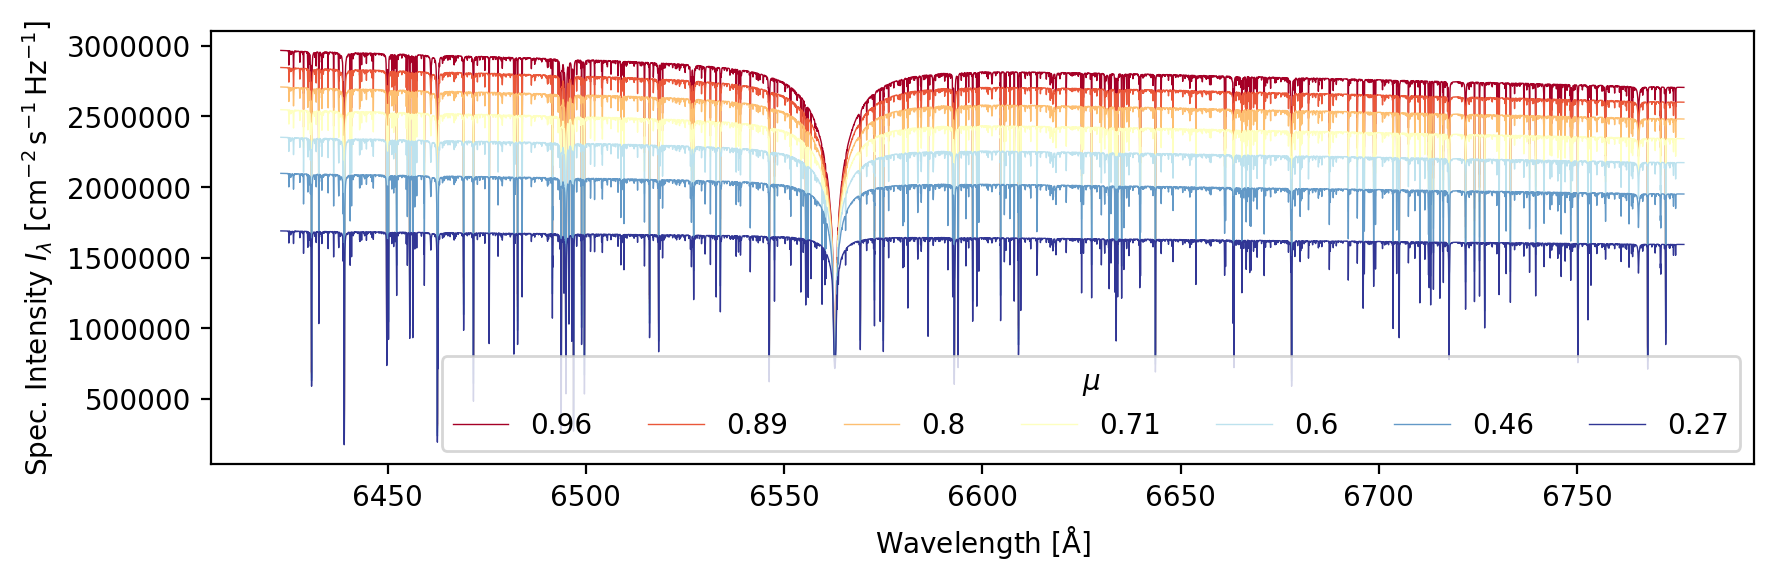
\includegraphics[width=\textwidth]{figures/solar_twin_specific_intensity.png}
 \caption{\textbf{Example output of \sme for a solar spectrum in HERMES CCD3 (around the Balmer $\mathrm{H}_\alpha$ line).} Shown are the the specific intensities (\texttt{sme.sint}) as a function of the equal-area midpoints of each equal-area annulus $\mu$.}
 \label{fig:sme_mu_output}
\end{figure}

We select small parts, that is 3D bins of the parameter space of \Teff, \logg, and \feh. For each of these parameters, we loop through the \marcs grid and compute randomly selected spectra within $\pm 1$ grid points in \Teff (with either $\pm 250$ or $\pm 100\K$), \logg ($\pm 0.5\dex$), and \feh ($\pm 1.0$, $\pm 0.5$ or $\pm 0.25\dex $).

\begin{figure}[hbt]
 \centering
 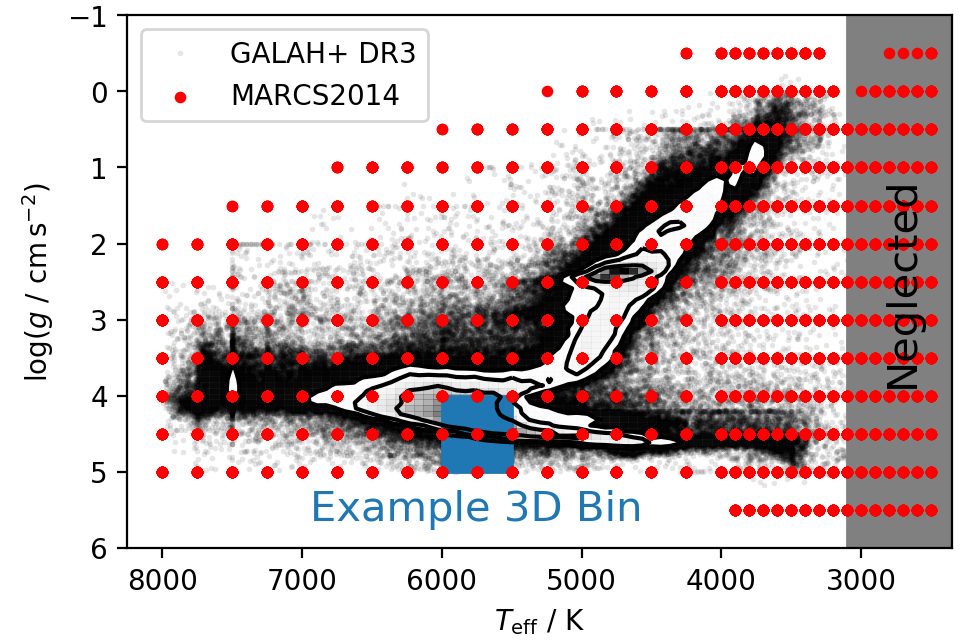
\includegraphics[width=\textwidth]{figures/teff_logg_grid_coverage.png}
 \caption{\textbf{Coverage in \Teff and \logg of MARCS2014 grid (red) and GALAH DR3 (black, including density countour).} Shown is also an example of one of the 3D bins used to create models with \TheCannon. MARCS grid points \Teff$ < 3100\K$ or \feh$<-3\dex$ are neglected throughout GALAH DR4.}
 \label{fig:teff_logg_grid_coverage}
\end{figure}

We explain the sampling of parameters and abundances in an exemplary way for the 3D bin centred on $T_\text{eff} = 5750\pm250\K$, $\log g = 4.5\pm0.5\dex$ and $\mathrm{[Fe/H]} = 0.0\pm0.25\dex$ (see blue box in Fig.~\ref{fig:teff_logg_grid_coverage}).

\begin{figure*}[ht]
 \centering
 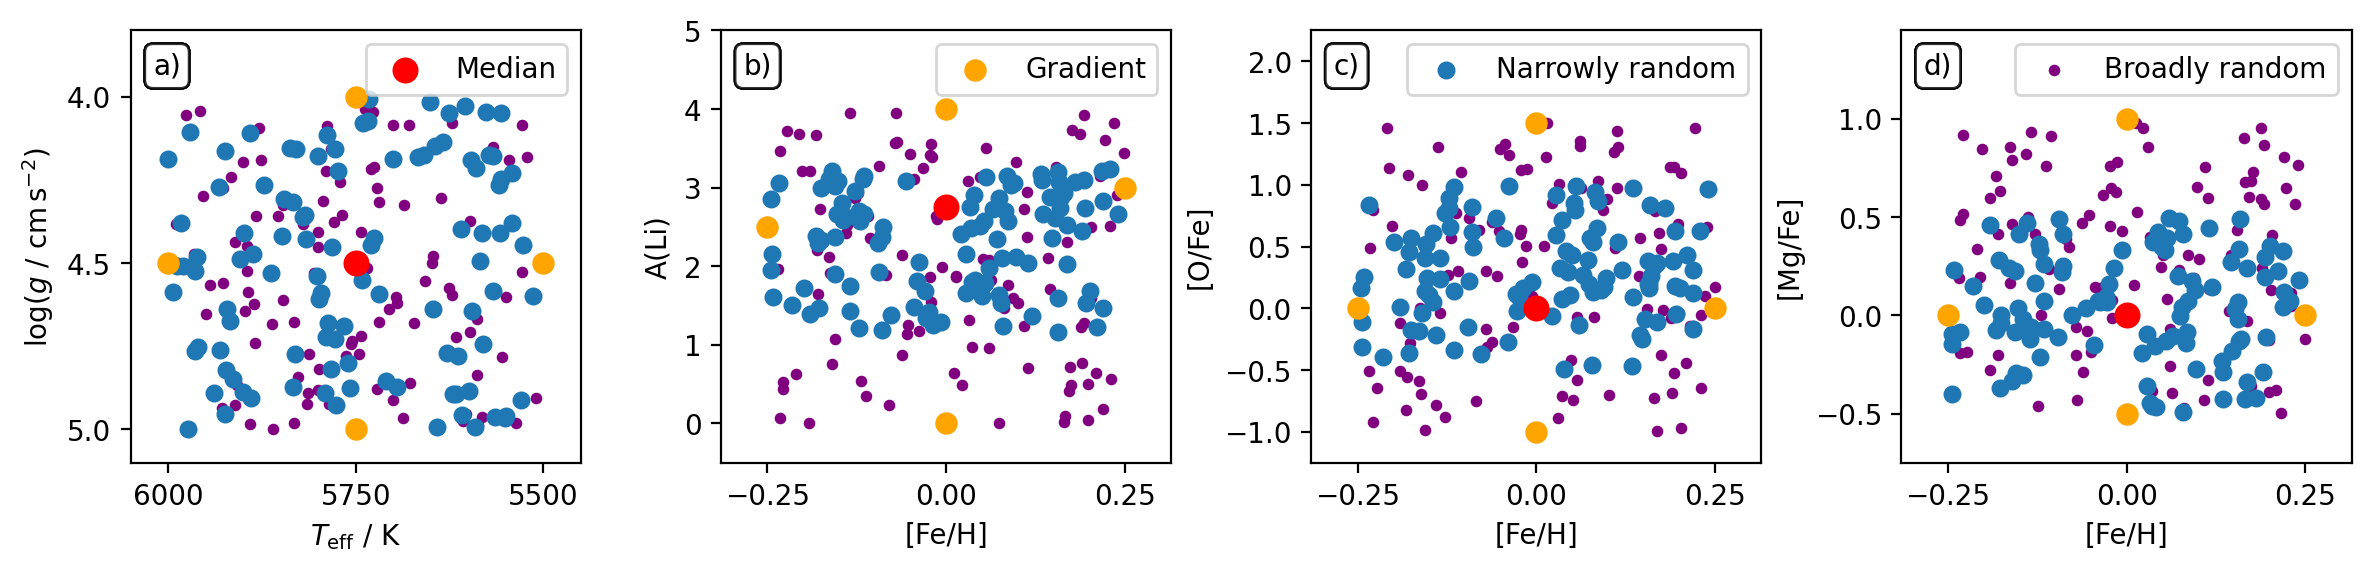
\includegraphics[width=\textwidth]{figures/example_3d_bin_sample.png}
 \caption{\textbf{Coverage of stellar parameters and abundances for one of the 3D bins.} Shown is the example of the solar 3D bin ($T_\mathrm{eff}~/~\mathrm{K} = 5750$, $\log (g~/~\mathrm{cm\,s^{-2}}) = 4.5$, $\mathrm{[Fe/H]}~/~\mathrm{dex} = 0.0$). \textbf{Panel a):} \Teff and \logg, \textbf{Panel b):} [Fe/H] vs. [Li/Fe], \textbf{Panel c):} [Fe/H] vs. [O/Fe], \textbf{Panel d):} [Fe/H] vs. [Mg/Fe]. While \Teff, \logg, and \feh are sampled randomly within the 3D bin, the abundances are sampled both narrowly (blue) and broadly (purple) within limits as described in the text. Red point indicate the median spectrum and orange points the adjusted spectra to test the gradient change of spectra with individual label.}
 \label{fig:example_3d_bin_sample}
\end{figure*}

For each synthetic spectrum to be computed within this 3D bin, the stellar parameters (\Teff, \logg, \feh, \vmic) and elemental abundances [X/Fe] of all 30 elements are randomly sampled within reasonable limits (see Eqs.~\ref{eq:sampling_teff}-\ref{eq:sampling_xfe}) and fed into \sme to create self-consistent synthetic spectra over the full wavelength range for \marcs atmospheres. 

An example of these sampled values is shown in Fig.~\ref{fig:example_3d_bin_sample} and samples from the following values:
\begin{align} 
    T_\text{eff}~/~\K &\in {5500..5750..6000} \\ \label{eq:sampling_teff}
    \log g~/~\dex &\in {4.0..4.5..5.0} \\
    \mathrm{[Fe/H]}~/~\dex &\in {-0.25..0.0..0.25} \\
    v_\text{mic}~/~\kms &\in Eq.~\ref{eq:vmic_initial} \\
    v \sin i~/~\kms &= 0\text{, but see Eq.~\ref{eq:vsini}} \\
    \mathrm{A(Li)} &\in \begin{cases} {1.05..2.75..3.26} \\ {0.00..4.00} \end{cases} \\
    \begin{array}{l}
    \mathrm{[X/Fe]~for~C,~N,~O, and}\\
    \mathrm{Y,~Ba,~La,~Ce,~Nd}
    \end{array}
    &\in \begin{cases} {-0.5..0.0..1.0} \\ {-1.0..1.5}  \end{cases} \\
    \mathrm{[X/Fe]~for~Mg,~Si,~Ti} &\in \begin{cases} {-0.5..0.0..0.5} \\ {-0.5..1.0}  \end{cases} \\
    \mathrm{[X/Fe]~for~all~other~elements} &\in \begin{cases} {-0.5..0.0..0.5} \\ {-1.0..1.0} \label{eq:sampling_xfe} \end{cases}
\end{align}

Based on the chosen \Teff and \logg, we calculate an initial value for \vmic within limits of $0.5$ to $4.0\kms$ based on Eq.~\ref{eq:vmic_initial} for $T_\text{eff}^\prime = T_\text{eff} - 5500\,\mathrm{K}$ as well as $\log g^\prime = \log g - 4.0$:
\begin{align} 
v_\text{mic} = \begin{array}{l}
1.198 + 3.16 \cdot 10^{-4} \cdot T_\text{eff}^\prime - 0.253 \cdot \log g^\prime \\ - 2.86\cdot 10^{-4} \cdot T_\text{eff}^\prime \cdot \log g^\prime + 0.165 \cdot \log g^\prime
\end{array} \label{eq:vmic_initial}
\end{align}
This relation is shifted by $+0.2\kms$ from the originally reported relation by \citet{DutraFerreira2016} based on 3D model atmospheres.

% \SB{Write equations for vmic from DR3 \citep{Buder2021} and \citet{DutraFerreira2016} as well as the requirement of at least 0.5 for the uniform sampling.}

For each spectrum, we first run a test on all available lines in the GALAH linelist, which is adapted from \citet{Heiter2021} and includes small changes to correct wrong $\log gf$ values for few lines within the GALAH wavelength range. We keep all atomic lines for the final synthesis and restrict the molecular lines to those with \textsc{sme}.depth above 0.001.

Spectra are computed at a resolution of $R = 300,000$ on a fine wavelength grid with 60,819 pixels spread over the extended wavelengths $4675.1- 4949.9$, $5624.1-5900.9$, $6424.1-6775.9$, and $7549.1-7925.9 \Angstroem$. We note that these extend significantly beyond the actual GALAH wavelength range.

We use 1D \marcs atmospheres from the \marcs grid \citep[][version 2014]{Gustafsson2008}, and interpolate them for combinations of \Teff, \logg, and \feh. We use grids of non-LTE departure coefficients by \citet{Amarsi2020} for H, Li, C, N, O, Na, Mg, Al, Si, K, Ca, Mn, and Ba. For all, except C, we use grids that include background scattering.

Our synthetic grid explicitly includes C and N abundances. C was previously included in the analysis of GALAH DR3, but limited to the atomic C line. The analysis thus neglected the molecular absorption features of $\mathrm{C_2}$ and CN at the beginning of CCD1 and end of CCD4, respectively. With the new self-consistent grid, we can however include these features, as they hold valuable information for both C and N, as well as several other features through the molecular equilibrium in stars \citep[see e.g.][]{Ting2018}.

To be able to test that the flux-label correlations found by our subsequent polynomial interpolation are limited to reasonable wavelength ranges, we also calculate one spectrum that is exactly in the middle of the parameter range and additional spectra, where we increase the value of one label at a time (e.g. increase [O/Fe] by $1\dex$) to test the response in the synthetic spectrum.

To save computational costs, we compute synthetic spectra with no rotational or macroturbulence broadening ($v_\text{mac} = v\sin i = 0\kms$), but save the model continuum flux (\texttt{sme.cmod}) and the specific intensities (\texttt{sme.sint}) as a function of the equal-area midpoints of each equal-area annulus $\mu$ (see Fig.~\ref{fig:sme_mu_output}). We then apply the broadening of spectra due to rotation (\vsini) with the flux integration code of the python-implementation \textsc{PySME} \citep{Wehrhahn2021} of \textsc{SME} \citep{Piskunov2017}. Depending on the expected rotational velocities (increasing with temperature) we sample a range of
\begin{align} \label{eq:vsini}
    v \sin i~/~\kms \in \{ 1.5, 3, 6, 9, 12, 18, 24^\star, 36^{\star \star}\}.
\end{align}

For bins with \Teff$\geq 5000\,\mathrm{K}$, we also include $v \sin i = 24 \kms$ and for those with \Teff$\geq 6000\,\mathrm{K}$ we also include $v \sin i = 36 \kms$. 
% The decision for these values was made based on the distribution of \vsini ($7.2_{-1.6}^{4.9}\kms$ with 90\% between 4.7 and $29.0\kms$) in GALAH+ DR3 \citep{Buder2021} and comparison with the grid values used by APOGEE DR16 \citep{Joensson2020}.

%%%%%%%%%%%%%%%%%%%%%%%%%%%%%%%%%%%%%%%%%%%%%%%%%%%%%%%%%%%%%%%%%%%%%%%%
\subsection{Interpolating synthetic spectra with neural networks} \label{sec:interpolating_synthetic_spectra_with_neural_networks}
%%%%%%%%%%%%%%%%%%%%%%%%%%%%%%%%%%%%%%%%%%%%%%%%%%%%%%%%%%%%%%%%%%%%%%%%

To allow a fast interpolation with new and different stellar labels, we use the method of training descriptive models to connect stellar fluxes at given pixels from a combination of stellar labels. This method is well established in stellar spectroscopy through the successful applications of quadratic models with \textit{The Cannon} \citep[see e.g.][]{Ness2015, Ness2016, Casey2016, Casey2017, Ho2017, Buder2018} as well as neural networks with \textit{The Payne} \citep[see e.g.][]{Ting2019, Xiang2019, Xiang2021}. Because of the needed flexibility\footnote{For a more detailed discussion on the advantages of neural networks for predicting spectra see \citet{Ting2019}.} to predict synthetic spectra with 36 stellar labels for a large parameter space, we are also choosing neural networks to interpolate between our synthetic spectra in this data release.

In particular, we use the neural network architecture and training algorithms of \textit{The Payne} \citep{Ting2019} for our data. We describe the connection of stellar labels $\boldsymbol{\ell}$ and the flux $f$ at each wavelength pixel $\lambda$ via
\begin{equation}
f_\lambda = w \cdot \sigma\bigg( \tilde{w}_\lambda^i \sigma \Big( w^k_{\lambda i} \ell_k + b_{\lambda i} \Big) + \tilde{b} \bigg) + \bar{f}_\lambda,
\label{eq:neural_network_function}
\end{equation}
where $\sigma$ is the Sigmoid function $\sigma (x) = 1/(1 + e^{-x})$ that encapsulates the so called layers of a neural network with $i = 300$ neurons \citep[see ][for more details]{Ting2019}. After optimising a loss function for $10^4$ steps, we consider the network trained with an optimised combination of three sets of weights and biases within the minimum and maximum ranges of each label. The trained networks can then be used with new input labels to quickly create synthetic spectra for the label optimisation.

%%%%%%%%%%%%%%%%%%%%%%%%%%%%%%%%%%%%%%%%%%%%%%%%%%%%%%%%%%%%%%%%%%%%%%%%%
\section{SINGLE SPECTRUM ANALYSIS (ALLSPEC)}
\label{sec:allspec_analysis}
%%%%%%%%%%%%%%%%%%%%%%%%%%%%%%%%%%%%%%%%%%%%%%%%%%%%%%%%%%%%%%%%%%%%%%%%%

As outlined in Sec.~\ref{sec:introduction}, the workflow of GALAH DR4 includes a first analysis step of all observed spectra without taking non-spectroscopic information for the optimisation. This allows to identify shifts of radial velocities between spectroscopic observations of the same stars\footnote{While repeat observations were only done for quality assurance in GALAH Phase 1, we have started to revisit a large amount of the fields for another 2x15 minuates to reach the updated needed exposure time for main GALAH fields of 1.5 hours.} and a more accurate co-adding of spectra for the \textit{allstar} analysis (see Sec.~\ref{sec:allstar_analysis}). Another motivation for this step is to get a first estimate of stellar labels without potentially biased photo- and astrometric, for example for binary stars.

The optimisation of stellar labels is thus aiming to minimise the absolute difference between synthetic and observed spectrum for all unmasked pixels, weighted by their uncertainty. Starting from a set of initial labels (Sec.~\ref{sec:initial_stellar_labels}), we create high-resolution synthetic spectra and downgrade them to the observed resolution and wavelength grid of each spectrum. In an important improvement of our analysis, we perform an on-the-fly re-normalisation of the observed spectrum, which allows a more accurate comparison of synthetic and observed spectra (Sec.~\ref{sec:comparison_synthetic_spectra_to_observations}) and thus a more accurate stellar label optimisation (see Sec.~\ref{sec:stellar_label_optimissation}).

%%%%%%%%%%%%%%%%%%%%%%%%%%%%%%%%%%%%%%%%%%%%%%%%%%%%%%%%%%%%%%%%%%%%%%%%%
\subsection{Initial stellar labels}
\label{sec:initial_stellar_labels}
%%%%%%%%%%%%%%%%%%%%%%%%%%%%%%%%%%%%%%%%%%%%%%%%%%%%%%%%%%%%%%%%%%%%%%%%%

% https://github.com/svenbuder/GALAH_DR4/blob/main/spectrum_analysis/galah_dr4_initial_parameters.ipynb

Initial values of all stellar labels are needed for creating a first synthetic spectrum. For \vrad, \Teff, \logg, and \vsini we use a combination of sources. Where possible, we use the previous estimates from GALAH DR3 GALAH DR3 \citep{Buder2021} and otherwise those from the GALAH DR4 reduction pipeline (Sec.~\ref{sec:spectroscopic_data_from_galah_observations}). Because of the limited accuracy of the latter for cool stars with $T_\text{eff} < 4000\,\mathrm{K}$ as well as the hottest stars with $T_\text{eff} > 6500\,\mathrm{K}$, we perform a consistency check with photometric information from $\Gaia$ DR3 \citep{Brown2021}, and 2MASS \citep{Skrutskie2006}. For most of the aforementioned cool and hot stars, we therefore prefer the parameters from the \Gaia DR3 photometric pipeline GSP-Phot \citep{Andrae2022,Fouesneau2022}.

In selected cases, we further adjust the starting parameters towards reasonable limits, for example for hot stars which are likely to be young and close to Solar [Fe/H]. Furthermore, we recalculate initial \vmic based on Eq.~\ref{eq:vmic_initial} and limits rotational broadening values to $3 \leq v \sin i \leq 10\,\mathrm{km\,s^{-1}}$ for stars below $T_\text{eff} = 5500\,\mathrm{K}$ and $3 \leq v \sin i \leq 20\,\mathrm{km\,s^{-1}}$ for hotter stars. The explicit choices of starting values for \Teff, \logg, \feh, \vmic, and \vsini are described in our \href{https://github.com/svenbuder/GALAH_DR4/blob/main/spectrum_analysis/galah_dr4_initial_parameters.ipynb}{online repository} and are depicted in Fig.~\ref{fig:initial_parameters}.

Based on the value of \feh we apply an offset to the $\mathrm{\alpha}$-elements O, Mg, Si, Ca, and Ti within our wavelength range. The initial value is 0.4 for $\mathrm{[Fe/H]} < -1$, 0.0 for $\mathrm{[Fe/H]} > 0$, and $-0.4\cdot \mathrm{[Fe/H]}$ for $-1 \leq \mathrm{[Fe/H]} \leq 0$. All other abundances are initialised at $\mathrm{[Fe/H]} = 0$.

%%%%%%%%%%%%%%%%%%%%%%%%%%%%%%%%%%%%%%%%%%%%%%%%%%%%%%%%%%%%%%%%%%%%%%%%%
\subsection{Comparison of synthetic spectra to observations}
\label{sec:comparison_synthetic_spectra_to_observations}
%%%%%%%%%%%%%%%%%%%%%%%%%%%%%%%%%%%%%%%%%%%%%%%%%%%%%%%%%%%%%%%%%%%%%%%%%

The major aim of our spectroscopic analysis is to predict the best set of stellar labels by minimising the uncertainty-weighted difference of observed and synthetic spectra. In this section, we describe several important steps to enable the pixel-level comparison of the higher resolution, oversampled synthetic spectra created with the neural networks from Sec.~\ref{sec:interpolating_synthetic_spectra_with_neural_networks} and the observational data at actually measured resolution and sampling (presented in Sec.~\ref{sec:spectroscopic_data_from_galah_observations}).

\subsubsection{Downgrading of synthetic spectra to observed resolution}

Because dedicated line-spread-function measurements are available for every spectrum (see Sec.~\ref{sec:spectroscopic_data_from_galah_observations}), we use this information to downgrade our synthetic spectra to the measured resolution of each observations. We then interpolate the over-sampled synthetic spectrum onto the observed wavelength.

\subsubsection{On-the-fly re-normalisation of observed spectrum}

Measurements of the GALAH flux and flux uncertainty are reported in counts by the reduction pipeline. To compare with our synthetic spectra, which are normalised to the continuum, we fit an outlier-robust polynomial function to the ratio of observed and synthetic spectrum and re-normalise our observed spectra and their uncertainties via this normalisation function.

This specific approach is similar to the internal routine of \textsc{SME} \citep{Piskunov2017} and has the important advantage, that no continuum points have to be defined. This is advantageous, because we try to cover the full parameter range of FGKM stars for which positions of continuum points -- corresponding to 1 on a (pseudo-)continuum-normalised spectrum -- differ significantly or for which continuum points may not even be present (as is the case for M stars).

We make two additional adjustments to the reduced spectra, which come in the form of counts and uncertainty per wavelength, $f_\lambda$ and $\sigma_{f,\lambda}$.

\begin{figure}[ht]
\centering
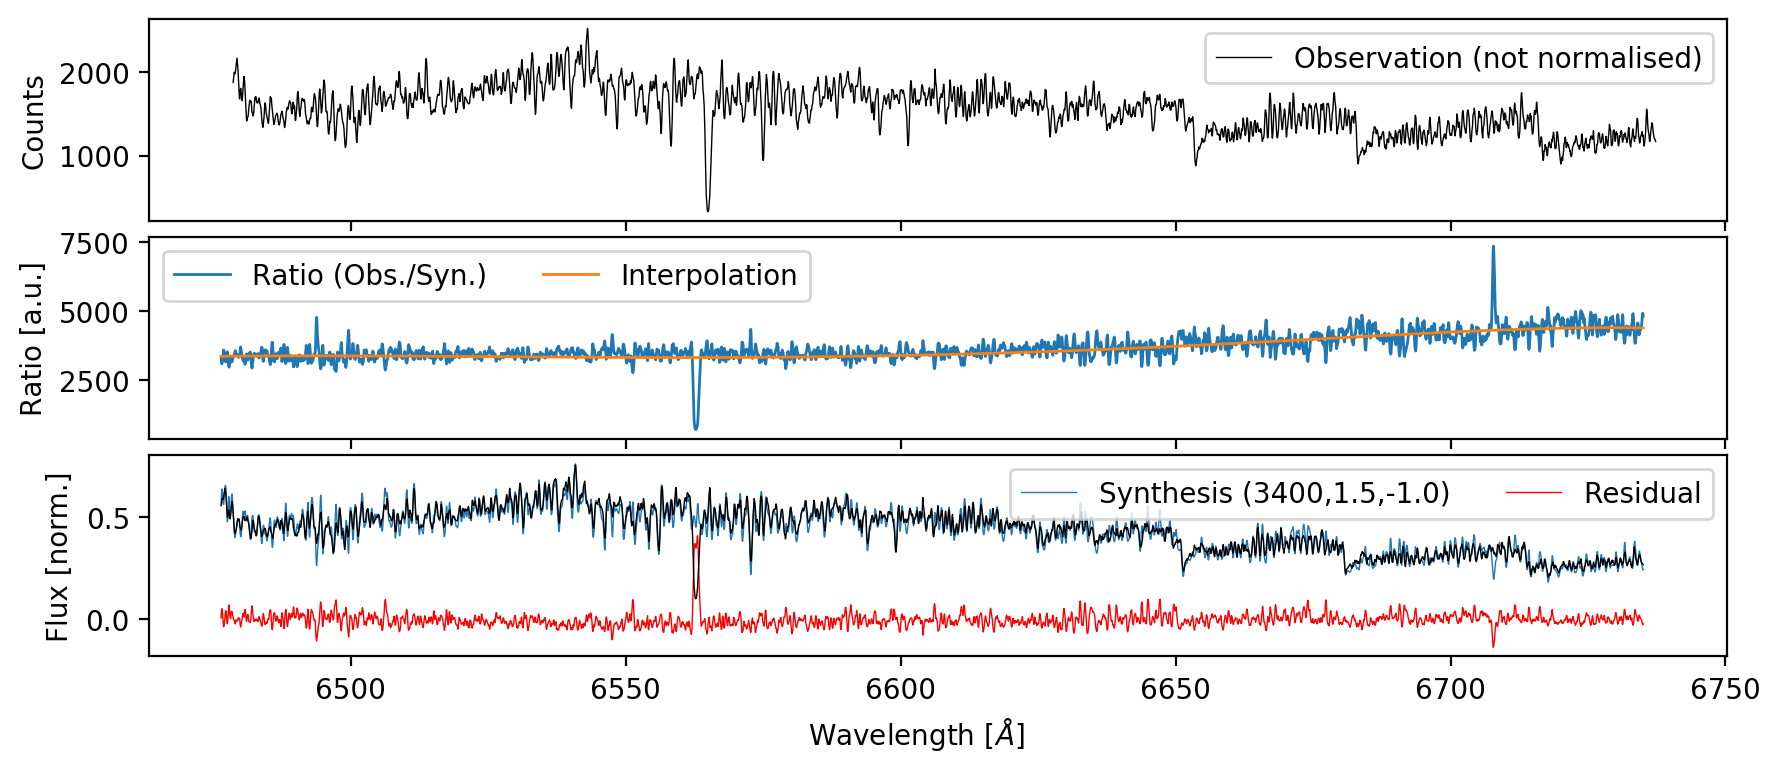
\includegraphics[width=\textwidth]{figures/Nuisance_example.png}
\caption{
\textbf{Example of normalisation for GALAH DR4 for a model spectrum that is selected during the label optimisation.}
\textbf{Panel (a):} Observed spectrum (counts) of star 2MASS XYZ.
\textbf{Panel (b):} Ratio (blue) of observed spectrum and model spectrum as well as Chebychev polynomial fit (orange).
\textbf{Panel (c):} Normalised observed spectrum (black) compared to the model spectrum (blue). Residuals (red) can then be used as input for the likelihood function.
}
\label{fig:ratio_normalisation}
\end{figure}

As we compare the observation to model spectra, we do not have to restrict ourselves to an a priory normalisation, but can take into account the residual information on the continuum in parts of the spectra. For each model spectrum that we compare to, we therefore perform a normalisation by fitting a Chebyshev polynomial with outlier clipping to the ratio of model and observation (see Fig.~\ref{fig:ratio_normalisation}). This allows us to both overcome previous shortcomings of the synthetic analysis in GALAH+ DR3 \citep{Buder2021}, which had to be restricted to small wavelength segments and assumed a linear relation for those. Our new approach allows us to properly assess the structure of deep and steep molecular features for cool stars, which dominate spectra of cool stars and carry significant information on \Teff as well as \vrad.

% \SB{Describe here the tests we do to make sure this actually provides a smooth transition between the different labels. Tests of the Cannon models show, that they can reproduce the spectra and their labels within for example $1\K$ \Teff, $0.01\dex$ \logg, and $0.01\dex$ \feh for the grid edges. But more thorough testing is needed.}
% \SB{Also keep in mind the issues found for \TheCannon with only 2 models applied to RAVE \citep{Casey2017}.}

%%%%%%%%%%%%%%%%%%%%%%%%%%%%%%%%%%%%%%%%%%%%%%%%%%%%%%%%%%%%%%%%%%%%%%%%%
\subsection{Stellar label optimisation}
\label{sec:stellar_label_optimissation}
%%%%%%%%%%%%%%%%%%%%%%%%%%%%%%%%%%%%%%%%%%%%%%%%%%%%%%%%%%%%%%%%%%%%%%%%%

In up to four major loops, we optimise the radial velocities and all other stellar labels and report a) their values, b) their co-variances, c) the best fit synthetic and re-normalised spectra along with their uncertainties and masks that indicate which pixels were used in the final optimisation.

Starting from the initial values, a first synthetic spectrum is computed and compared with the observation in order to assess the initial radial velocity. This is done by applying the \textsc{scipy.signal.find\_peaks} algorithm on a the residuals\footnote{We use the inverse of the residuals that were normalised with the smallest residual values.} of non-shifted observed and synthetic spectra, when the latter is shifted by $v_\text{rad} = -1000..(2)..1000\kms$ (see Fig.~\ref{fig:181221003101356_single_fit_rv}a). If no peak is found, the initial \vrad value is used hereafter. If more than one peak is found (see Fig.~\ref{fig:181221003101356_single_fit_rv} with \Gaia DR3 agreeing with the systemic radial velocity), the two strongest peaks are reported and trigger a stellar label estimation assuming binary star (Sec.~\ref{sec:binary_analysis}. For the purpose of the single star analysis, a narrower search is conducted around the highest peak with a \vrad shift of $-20.00..(0.04)..20.00\kms$ around said peak by fitting a Gaussian function to the inverse of the residuals that were normalised with the smallest residual values (see Fig.~\ref{fig:181221003101356_single_fit_rv}c). The mean of this fit and its uncertainty are reported by the pipeline.

\begin{figure}[hbt]
\centering
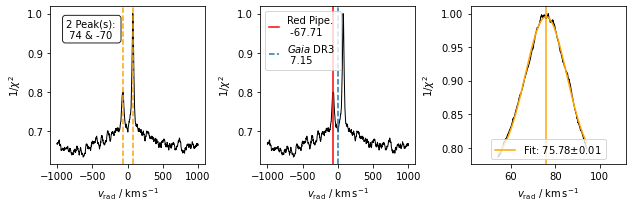
\includegraphics[width=\textwidth]{figures/181221003101356_single_fit_rv.png}
\caption{\textbf{Output of the radial velocity fitting module.} \textbf{Panel a)} shows the initial broad search on a \vrad array of $-1000..(2)..1000\kms$. In the case of 2MASS J06084657-7815235, two peaks (yellow, dashed) are visible for this line-splitting spectroscopic binary. \textbf{Panel b)} shows the same plot, but overlaid with the GALAH DR4 reduction pipeline (red) and \Gaia DR3 (blue, dashed) estimates. \textbf{Panel c)} shows the narrow window of $-20.00..(0.04)..20.00\kms$ around the highest peak and the Gaussian fit (yellow) to it.}
\label{fig:181221003101356_single_fit_rv}
\end{figure}

The centerpiece of our optimisation is the \textsc{scipy.optimise} routine \textsc{curve\_fit} module \citep{scipy}, which we call with counts and uncertainties (our absolute sigmas) as input for a placeholder function that self-consistently re-normalises the observed spectrum. We estimate the labels via the least squares optimisation within less than $10^4$ iterations and a desired relative error (\texttt{xtol}) below 0.0001.

For the each optimisation loop, a new, best-fit 3D bin and neural network is identified via a grid search in the \TLF dimensions with \textsc{sklearn.cKDtree}. If the stellar labels that are being fitted have changed (for example if an element is deemed not detectable for the new 3D bin), the label and its value is either deleted or initialised with $\mathrm{[X/Fe]} = 0$.

While the optimisation has not converged (the final parameters \TLF are not within the current 3D bin), the optimisation is repeated, starting with the previous best-fit parameters as starting guesses.

\subsubsection{Which labels are optimised?} \label{sec:which_labels_are_optimised}

%% This paragraph is based on the combination of 
%% spectrum_interpolation/galah_dr4_grid_interpolation_recommend_labels.ipynb
%% and
%% spectrum_analysis/galah_dr4_spectrum_analysis_single.ipynb

As part of the synthetic grid computations, we have perturbed each label individually to our chosen maximum and minimum ranges (see Sec.~\ref{subsubsec:spectrum_grid}). This allows us to also judge which stellar labels to fit for each given star. We choose to fit a stellar label, if either of the two cases applies to said label for the GALAH wavelength range when neglecting the cores of the Balmer lines: Does the spectrum between minimum and maximum label value at any pixel change more than a certain threshold (0.07 of the normalised spectrum)? Does the spectrum between minimum and maximum label value change by more than 0.005 of the normalised spectrum for at least 25\% of the spectrum? While the first case is constructed for atomic lines, such as \ion{Li}{i} 6708, the second case is addressing in particular molecular lines like the $\mathrm{C_2}$ and $\mathrm{CN}$ lines. For spectra that are missing the infrared arm (CCD4) we exclude the otherwise possibly fit labels for N, O, L, and Rb.

Initial tests of the pipeline have revealed that in cases where the initial parameter guesses are deviating significantly from the final ones, several elemental abundance estimates were shifted towards their boundaries, leading to a masking of their elemental abundances lines by the masking module (Sec.~\ref{sec:masking_of_unreliable_wavelength_regions}) at the beginning of each optimisation loop. To minimise this effect, we therefore shift the interim abundance values towards the narrow label boundaries. In practise, we this limit the initial and interim abundances to 1.05..3.26 for A(Li), $\mathrm{[X/Fe]} = -0.5..1.0$ for C, N, O, Y, Ba, La, Ce, and Nd, and $\mathrm{[X/Fe]} = -0.5..0.5$ for all other elements before optimising them again. For warm and hot stars ($T_\text{eff} > 6000\K$), this effect was seen to effect multiple abundances, such that we needed to implement a zeroing of all abundances (except Lithium) for stars above $6000\K$, which would on average be expected to be young and have a solar-like composition.

\begin{figure*}[ht]
\centering  
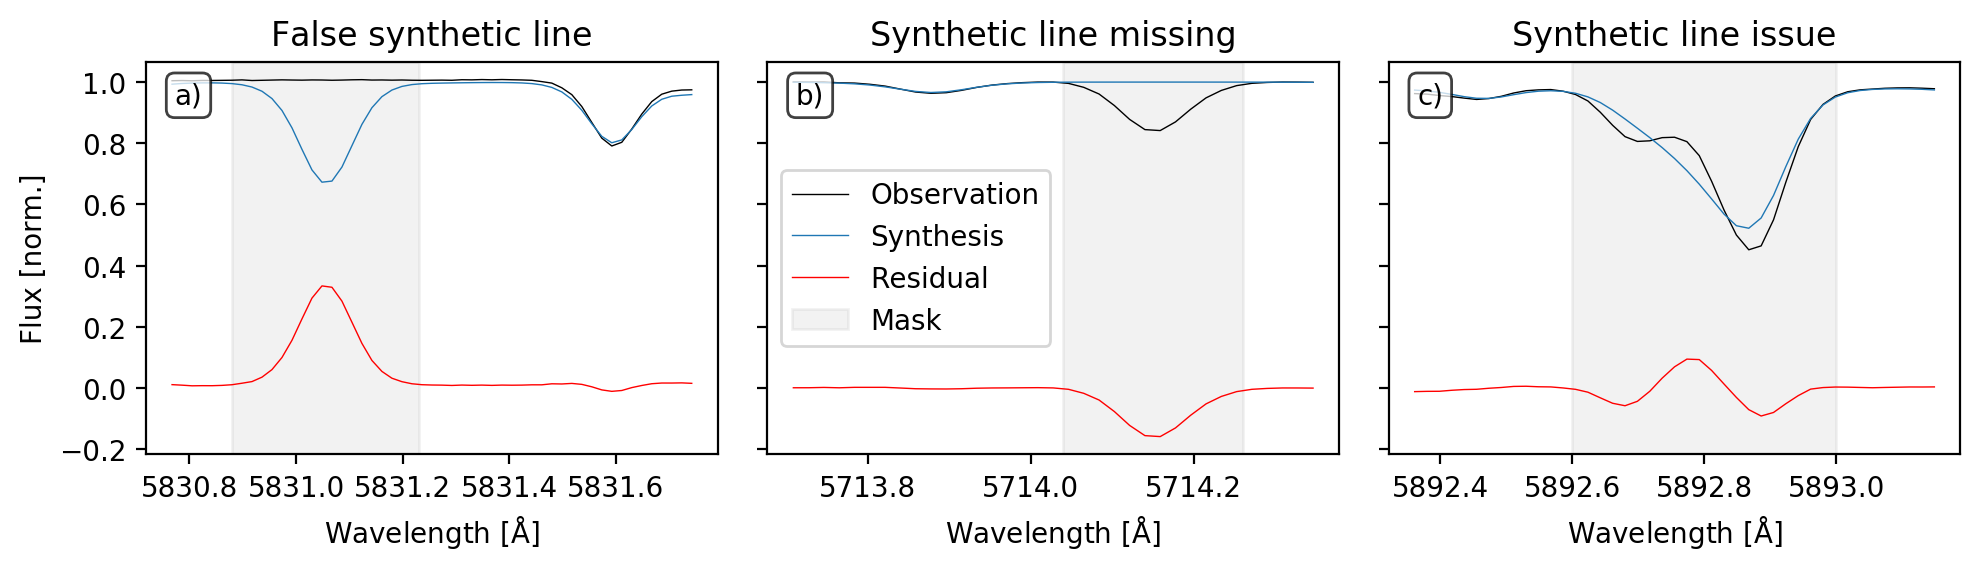
\includegraphics[width=\textwidth]{figures/example_masking_sun.png}
\caption{\textbf{Examples of masks applied to unreliable pixels for the spectrum fitting, that is the minimisation of residuals (red) between observation (black) and synthesis (blue).} \textbf{Panel a)} showing a strong synthetic line, where no line is observed in the Sun. \textbf{Panel b)} showing an observed line without any line being synthesised. \textbf{Panel c)} showing significant disagreement between the two observed lines and the synthesis.} \label{fig:example_masking_sun}
\end{figure*}

\subsubsection{Masking of unreliable wavelength regions} \label{sec:masking_of_unreliable_wavelength_regions}

Not all pixels of the observed or synthetic spectra might prove useful for estimating reliable stellar labels. Observations can include bad pixels/patterns and incorrect corrections (for example of telluric or sky lines). Flux predictions of synthetic spectra are only as good as the input physics (limited for example for specific lines via uncertain oscillator strengths).

% Based on https://github.com/svenbuder/GALAH_DR4/blob/main/spectrum_analysis/galah_dr4_solar_analysis.ipynb
To minimise the influence of inaccurate synthetic pixel predictions, we have compared a 2dF-HERMES observation of the asteroid 4~Vesta and a high-quality  Solar spectrum by \citet{Hinkle2000} with the flux that would be predicted through our pipeline for a star with Solar labels ($T_\text{eff} = 5772\K$, $\log g = 4.438\dex$, $\mathrm{[Fe/H]} = 0.00\dex$, $v_\text{mic} = 1.06\kms$, $v \sin i = 1.6\kms$, $v_\text{mac} = 4.2\kms$ \citep{Prsa2016, Jofre2017}, and $\mathrm{[X/Fe]} = 0.00\dex$ for the default Solar abundance pattern for \marcs by \citet{Grevesse2007}).

We have identified all lines that showed differences of the normalised flux of more than $0.1$, lines where either a synthetic line or an observed one was completely missing, or lines that were significantly misaligned. Examples of this \href{https://github.com/svenbuder/GALAH_DR4/blob/main/spectrum_analysis/spectrum_masks/solar_spectrum_mask.fits}{list} of masks are shown in Fig.~\ref{fig:example_masking_sun}. To avoid the influence of bad spectrum regions with an observational origin, we mask pixels where the synthetic and re-normalised observed spectrum differ by more than $5\sigma$ or a flux of 0.3 (0.4 before the initial optimisation). To avoid the masking of lines that are vital for our spectroscopic analysis, we have created a \href{https://github.com/svenbuder/GALAH_DR4/blob/main/spectrum_analysis/spectrum_masks/vital_lines.fits}{list} with segments of such lines that is mainly based on the previous element masks from GALAH DR3 \citep{Buder2021}. The final mask of pixels to use for the optimisation then includes all vital line regions and those wavelengths that are not unreliable in the synthesis show a too strong disagreement between observation and synthesis.

In addition to this default masking, we exclude pixels for each major iteration, for which the flux of observation and synthetis differ by more than $5 \sigma$ and 0.3 of the normalised flux and by more than 1 for the vital line regions.

We further indirectly take into account the currently less constrained molecular data for cool stars in optical spectra, in particular towards the blue \citep[e.g.][]{Rains2021}. For presumably cool stars (with initial $T_\text{eff} < 4100\,\mathrm{K}$), we therefore double the observational uncertainty of the blue arm.

%%%%%%%%%%%%%%%%%%%%%%%%%%%%%%%%%%%%%%%%%%%%%%%%%%%%%%%%%%%%%%%%%%%%%%%%%
\section{SINGLE STAR ANALYSIS (ALLSTAR)}
\label{sec:allstar_analysis}
%%%%%%%%%%%%%%%%%%%%%%%%%%%%%%%%%%%%%%%%%%%%%%%%%%%%%%%%%%%%%%%%%%%%%%%%%

After spectroscopic estimates are computed for all spectra (Sec.~\ref{sec:allspec_analysis}), all spectra of the same star are co-added and re-analysed while taking into account photometric and astrometric information to constrain the surface gravities. This approach was already very succesfully applied for GALAH DR3 \citep{Buder2021} with \Gaia DR2 distances \citep{BailerJones2018} to overcome spectroscopic degeneracies.

We explain the implementation of the self-consistent surface gravities into the fitting routine in Sec.~\ref{sec:logg_phot}.

\subsection{Self-consistent surface gravities} \label{sec:logg_phot}

We can estimate the logarithmic surface gravity, $\log g$, as a combination of its definition ($g \propto \frac{\mathcal{M}}{\mathcal{R}^2}$) and the Stefan-Boltzmann law relative to the Solar values:
\begin{equation}
\log g = \log g_\odot + \log \frac{\mathcal{M}}{\mathcal{M_\odot}} + 4 \log \frac{T_\mathrm{eff}}{T_\mathrm{eff,\odot}} - \log \frac{L_\mathrm{bol}}{L_\mathrm{bol,\odot}} \label{eq:logg}
\end{equation}

While we can use our spectroscopically determined $T_\mathrm{eff}$, the other values have to be estimated through models or non-spectroscopic information. The logarithmic bolometric luminosity, $L_\mathrm{bol}$, can be estimated from the bolometric magnitude, such that $\log \frac{L_\mathrm{bol}}{L_\mathrm{bol,\odot}} = -0.4 \cdot \left(M_\mathrm{bol} - M_\mathrm{bol,\odot} \right)$. The bolometric magnitude can be estimated from any given apparent magnitude, if we correct the latter by the distance modulus, bolometric correction, and extinction. Because for essentially all stars of GALAH DR4, we have outstanding infrared magnitudes available which suffer less from (uncertain) extinction corrections, we continue to chose $K_S$ as the magnitude to estimate our bolometric magnitudes and luminosities via
\begin{equation}
M_\mathrm{bol} = K_S - 5\cdot \log \frac{D_\varpi}{10} + BC(K_S) - A(K_S). \label{eq:mbol}
\end{equation}

While the values for $K_S$, $D_\varpi$, and $A(K_S)$ are readily available (see Sec.~\ref{sec:non-spec_data}), we need to estimate the bolometric correction from tabulated values using the routines provided by \citet{Casagrande2018}:
\begin{equation}
BC(K_S) = f(T_\mathrm{eff}, \log g, \mathrm{[Fe/H]})
\label{eq:bc_ks}
\end{equation}
We choose to assume an extinction value of $E(B-V) = 0\,\mathrm{mag}$ for this particular interpolation and post-correct the value by $A(K_S)$ our actual extinctions can exceed the tabulated values of $E(B-V) = 0.72\,\mathrm{mag}$ by \citet{Casagrande2018} and our available $E(B-V)$ values from \citet{Schlegel1998} are upper limits that can overestimate the actual extinction of our observed targets.

Because of the appearance of $\log g$ in Eq.~\ref{eq:bc_ks}, we iterate the calculation of $BC(K_S)$ and subsequently $\log g$ up to four times or until the latter value changes less than $0.02\,\mathrm{dex}$ between iterations. Similarly, we need to estimate the stellar masses (and ages as a byproduct) from tabulated values, that is,
\begin{equation}
\mathcal{M}, \tau = f(T_\mathrm{eff}, \log g, \mathrm{[Fe/H]}, L_\mathrm{bol,\odot})
\label{eq:mass_age}
\end{equation}
For this on-the-fly estimate of masses and ages we use an earlier version of the \texttt{ELLI} code by \cite{Lin2018} for a likelihood-weighted estimate with default uncertainties of $100\,\mathrm{K}$, $0.25\,\mathrm{dex}$, $0.2\,\mathrm{dex}$, and an average uncertainty of $L_\mathrm{bol,\odot}$ from propagated uncertainties of Eq.~\ref{eq:mbol}.

We interpolate over the detault tables of {\sc parsec+colibri} isochrones \citep{Bressan2012, Marigo2017} from that cover the logarithmic ages of $\log (\tau~/~\mathrm{Gyr}) = 8.00..(0.01)..10.18$ by default and metallicities $\mathrm{[M/H]} = -2.75..(0.25)..-0.75$ as well as $\mathrm{[M/H]} = -0.6..(0.1)..0.7$. For open clusters with age estimates below $1\,\mathrm{Gyr}$ as well as unevolved stars that are more luminous than expected from the oldest cool main sequence isochrone with matching $\mathrm{[M/H]}$, we sample $\log (\tau~/~\mathrm{Gyr}) = 6.19..(0.01)..10.18$. We exclude hot stars above $10\,000\,\mathrm{K}$ as well as extremely evolved stars ($\log g > 6\,\mathrm{dex}$ or $J - K_S > 2\,\mathrm{mag}$) as they fall far outside our spectroscopic pipeline range. We convert between the theoretical [M/H] and our measured [Fe/H] as well as $\mathrm{[\upalpha/Fe]}$ via the correlation by \citet{Salaris2006}, $\mathrm{[M/H]} = \mathrm{[Fe/H]} + \log\left(10^{\mathrm{[\upalpha/Fe]} \cdot 0.694 + 0.306} \right)$.

%%%%%%%%%%%%%%%%%%%%%%%%%%%%%%%%%%%%%%%%%%%%%%%%%%%%%%%%%%%%%%%%%%%%%%%%%
\section{BINARY STAR ANALYSIS (BINARY)}
\label{sec:binary_analysis}
%%%%%%%%%%%%%%%%%%%%%%%%%%%%%%%%%%%%%%%%%%%%%%%%%%%%%%%%%%%%%%%%%%%%%%%%%

% spectrum_analysis/galah_dr4_spectrum_analysis_binary.ipynb

Motivated by the extensive study of GALAH binary star spectra by \citet{Traven2020}.

In our strictly spectroscopic implementation, we only use the stellar GALAH spectra and the two radial velocity peaks identified in the radial velocity optimisation step (see Fig.~\ref{fig:181221003101356_single_fit_rv}) of the single star analysis (Sec.~\ref{sec:allspec_analysis}).

Fitting RV1, RV2, Teff1, Teff2, logg1, logg2, FeH, vmic1, vmic2, vsini1, vsini2


\newpage
%%%%%%%%%%%%%%%%%%%%%%%%%%%%%%%%%%%%%%%%%%%%%%%%%%%%%%%%%%%%%%%%%%%%%%%%%
\section{POST-PROCESSING}
\label{sec:post_processing}
%%%%%%%%%%%%%%%%%%%%%%%%%%%%%%%%%%%%%%%%%%%%%%%%%%%%%%%%%%%%%%%%%%%%%%%%%

%%%%%%%%%%%%%%%%%%%%%%%%%%%%%%%%%%%%%%%%%%%%%%%%%%%%%%%%%%%%%%%%%%%%%%%%%
\subsection{Stellar parameter flags \textsc{flag\_sp}}
\label{sec:flag_sp}
%%%%%%%%%%%%%%%%%%%%%%%%%%%%%%%%%%%%%%%%%%%%%%%%%%%%%%%%%%%%%%%%%%%%%%%%%

Fig.~\ref{fig:examples_flag_sp}



\begin{figure*}[ht]
 \centering
 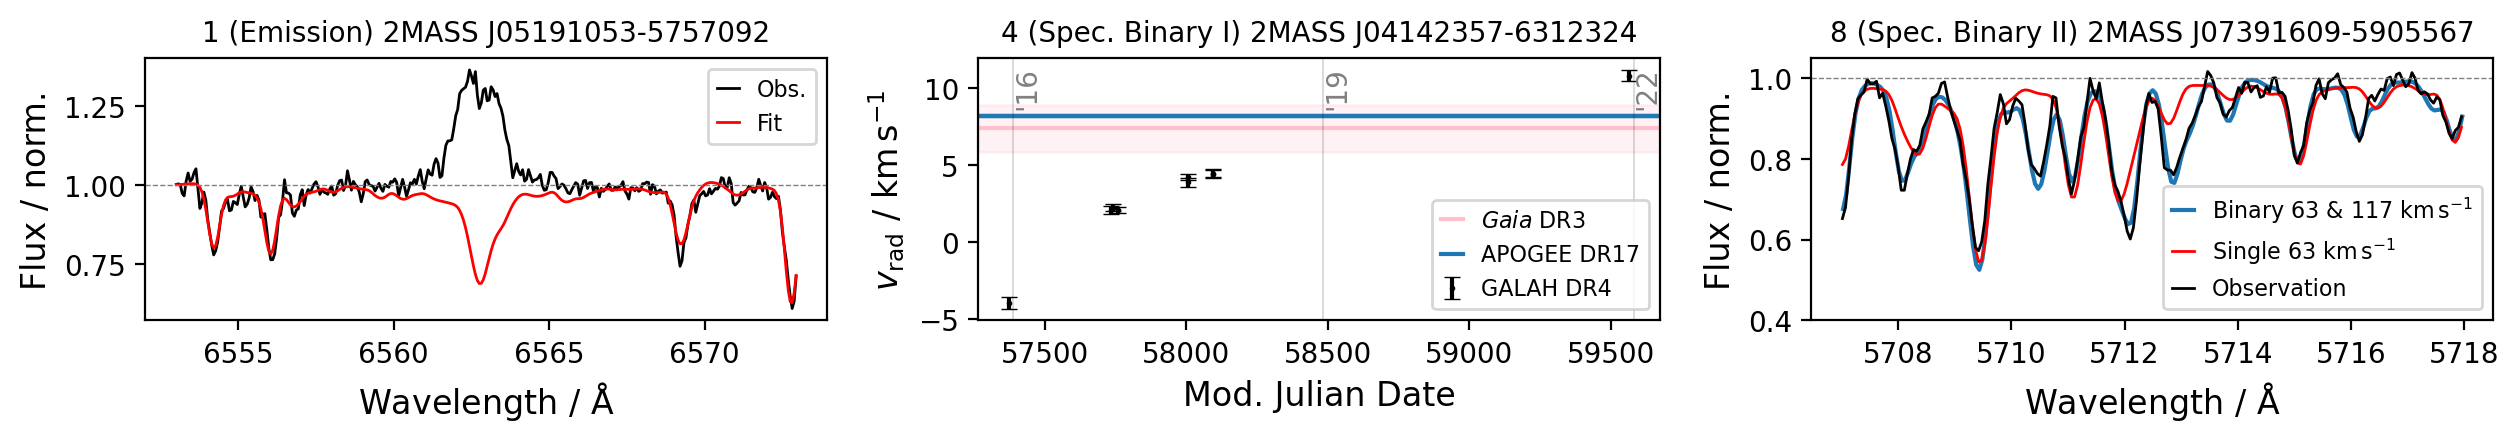
\includegraphics[width=\textwidth]{figures/examples_flag_sp.png}
 \caption{\textbf{Examples of stars with raised major quality flag \texttt{flag\_sp}.}
 \textbf{Panel a)} shows the spectrum of a star with Balmer lines in emission. \textbf{Panel b)} shows an example of a spectroscopic binary (SB) of type I (no line split) with changing radial velocity between observations. \textbf{Panel c)} shows the spectrum of a line-splitting binary (SB type II) which is better fit with our binary fitting algorithm.} \label{fig:examples_flag_sp}
\end{figure*}

Fig.~\ref{fig:teff_logg_vsini}

\begin{figure*}[ht]
 \centering
 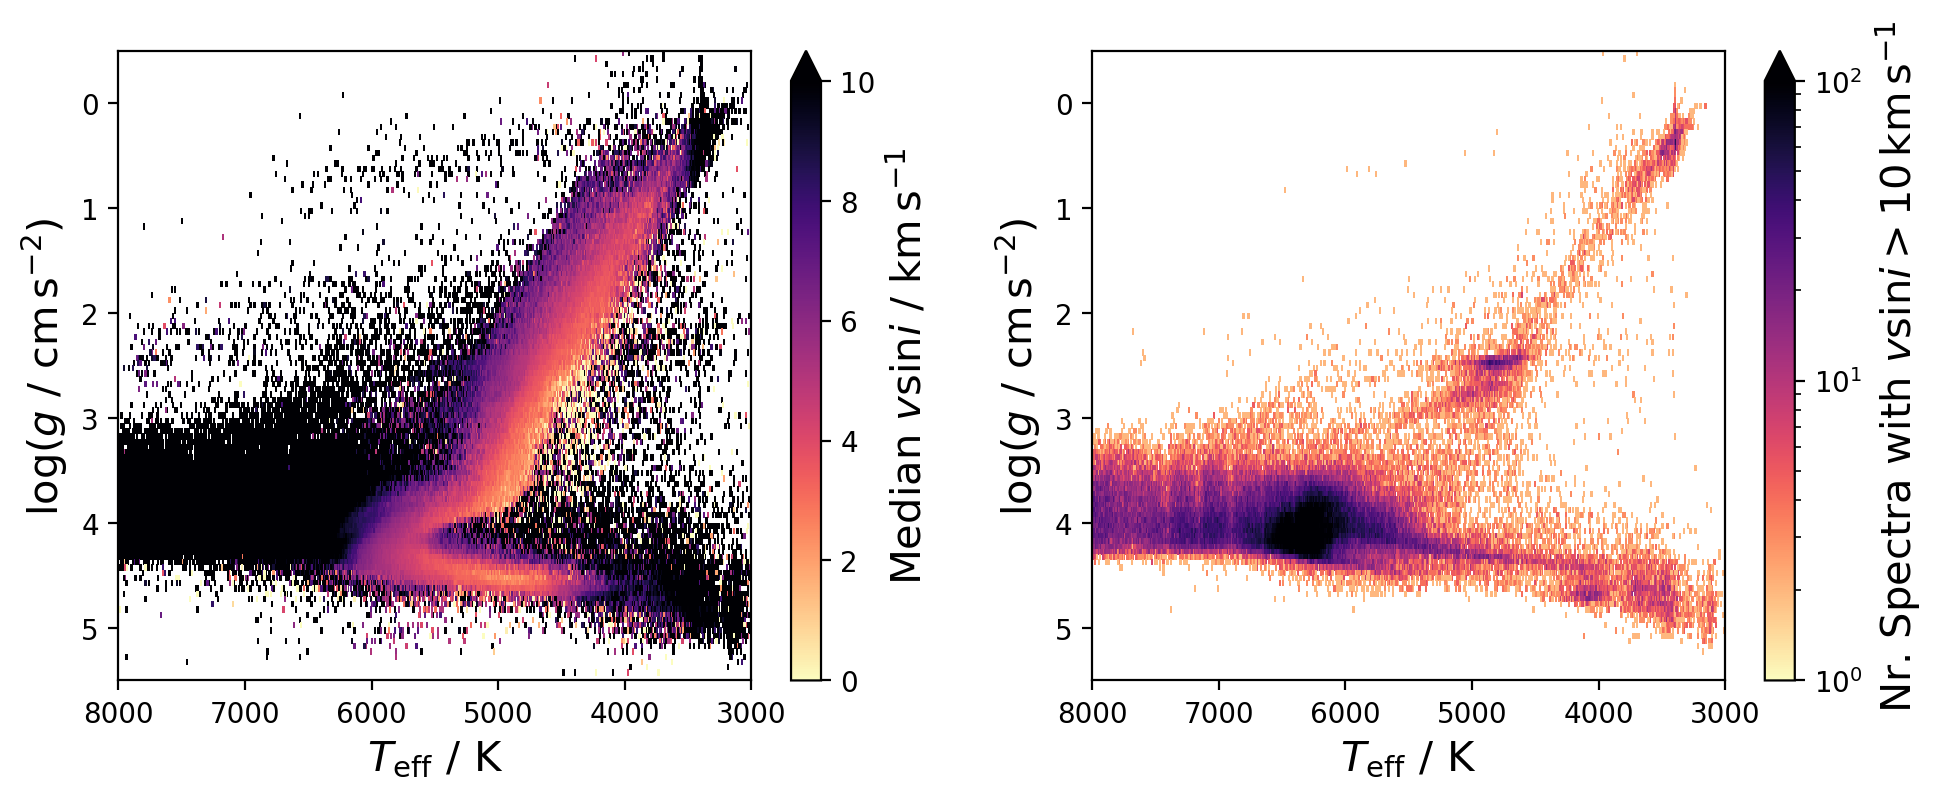
\includegraphics[width=\textwidth]{figures/teff_logg_vsini.png}
 \caption{
 \textbf{Overview of rotational velocity of stars}
} \label{fig:teff_logg_vsini}
\end{figure*}

Issues with wavelength solution: 170509
CRVAL flag 2 for dates around 190204, 190205
CRVAL flag 8 for dates 170828, 170829, 170904, 190204, 190205

Forgot to run dates 170128,171230,180126


%%%%%%%%%%%%%%%%%%%%%%%%%%%%%%%%%%%%%%%%%%%%%%%%%%%%%%%%%%%%%%%%%%%%%%%%%
\subsection{Abundance detection or upper limit}
\label{sec:abundance_detection_or_upper_limit}
%%%%%%%%%%%%%%%%%%%%%%%%%%%%%%%%%%%%%%%%%%%%%%%%%%%%%%%%%%%%%%%%%%%%%%%%%

To assess if the abundance estimates are a true detection or an upper limit for element X, we produce synthetic spectra with the same stellar labels, but decrease the abundance [X/Fe] to the lower limit of the neural network (or decrease the [Fe/H] value by -0.5 for Fe). The residuals in units of sigma between the best-fit spectrum and spectrum with lowest possible [X/Fe] or lowered [Fe/H] then allow us to identify a detection (with maximum differences beyond 3 sigma) or upper limits. We note again that our initial test of overall detectability (Sec.~\ref{sec:which_labels_are_optimised}) allowed us identify elements for which not even an upper limit was expected.

%%%%%%%%%%%%%%%%%%%%%%%%%%%%%%%%%%%%%%%%%%%%%%%%%%%%%%%%%%%%%%%%%%%%%%%%%
\subsection{Elemental abundance flags \textsc{flag\_x\_fe}}
\label{sec:flag_x_fe}
%%%%%%%%%%%%%%%%%%%%%%%%%%%%%%%%%%%%%%%%%%%%%%%%%%%%%%%%%%%%%%%%%%%%%%%%%

1: upper limit \\ 
2: no measurement available\\
4: no convergence\\
8: measurement above limit\\
16: measurement below limit\\
32: measurement issue of CNO: $\mathrm{[C/N]} < -1$ for non-giants ($T_\text{eff} > 5500\,\mathrm{K}$ or $\log g > 3.5$) or no $\mathrm{[N/Fe]}$ measured for non-giants ($T_\text{eff} > 5500\,\mathrm{K}$ or $\log g > 3.5$) -> raising flag of $\mathrm{[C/Fe]}$ in that case as well as
$\mathrm{[N/Fe]}$ extended non-giants ($T_\text{eff} > 5750\,\mathrm{K}$ or $\log g > 4.$ -> raising flag of $\mathrm{[N/Fe]}$
64: measurement of Li, Ca, or Ba when CCD3 wavelength seems to be off (cdelt beyond the usual range of xx-xx) \\

% problematic_cfe = (
%     # [C/N] < -1 for non-giants
%     (
%         (data['c_fe'] - data['n_fe'] < -1) & # [C/N] < -1
%         ~((data['logg'] < 3.5) & (data['teff'] < 5500)) # not_giant
%     ) |
%     # No [N/Fe] for non-giants
%     (
%         (data['flag_n_fe'] == 2) & # no [N/Fe]
%         ~((data['logg'] < 3.5) & (data['teff'] < 5500)) # not_giant
%     )
% )


% ['*Bitmask* | *Description* | '],
%  [':--------------|:--------------|'],
%  ['0 | No flag rasied | '],
%  ['1 | Upper limit | '],
%  ['2 | No measurement available | '],
%  ['4 | No convergence | '],
%  ['8 | Measurement above limit: A(Li) > 4; [X/Fe] > 1.5 for C,N,O,Y,Ba,La,Ce,Nd; [X/Fe] > 1.0 for the rest | '],
%  ['16 | Measurement below limit: A(Li) < 0; [X/Fe] < -0.5 for Mg, Si, Ti; [X/Fe] < -1.0 for the rest | '],
%  ['32 | Measurement issue of CNO | ']



%Our pipeline will find the most suitable model and in particular set of abundances for the given observation. That does, however, not necessarily mean that the abundance of each element is actually well determined, because lines of the element may actually not be detected. For each element, we therefore run a post-processing routine to estimate if the measured abundance is indeed significant compared to the uncertainty of the spectrum. For each star, we therefore take the best-fit labels and neural network model and assess the change in the model spectrum when changing one abundance at a time to the lower boundary of the neural network model. If the difference between the spectrum of the best-fit and the lowest possible abundance is not above $3\sigma$ for a given elemental label, we do not consider it a reliable detection and thus raise the flag \textsc{flag\_x\_fe} for this label.
%
%% see https://github.com/svenbuder/GALAH_DR4/blob/main/spectrum_analysis/galah_dr4_spectrum_analysis_single.py
%
%%%%%%%%%%%%%%%%%%%%%%%%%%%%%%%%%%%%%%%%%%%%%%%%%%%%%%%%%%%%%%%%%%%%%%%%%%
%% \subsection{Goodness of fit}
%% \label{sec:goodness_of_fit}
%%%%%%%%%%%%%%%%%%%%%%%%%%%%%%%%%%%%%%%%%%%%%%%%%%%%%%%%%%%%%%%%%%%%%%%%%%
%
%% Raise flag\_sp by 4
%
%% \subsection{Rotational broadening}
%
%% vsini only provided from 1.5 to 24.
%
%% Values below 0 and above 25 raise flag\_sp b 8
%
%% \subsection{Emission lines}
%
%% We use the composite trapezoidal rule to estimate equivalent width for emission based on the difference between observed and model spectrum around $2\,\mathrm{\AA}$ of each Balmer line. We flag the spectrum (raising flag\_sp by 16), if the observed spectrum is without a doubt in emission with a median observed flux above zero for the Balmer line cores ($\pm 0.5\,\mathrm{\AA}$ of the line center).
%
%% \subsection{Flagging of problematic measurements}
%
%% \SB{Flag if parameters outside of the range of \TheCannon (e.g. \vsini$ > 30 \kms$, see Sec.~\ref{subsubsec:polynomials})}
%
%% \SB{Flag if parameters are outside of convex hull of isochrone grid, when using photoastrometric information. Also note that we have cut away \Teff above $10,000\K$ and \logg above $6\dex$.}

\newpage
%%%%%%%%%%%%%%%%%%%%%%%%%%%%%%%%%%%%%%%%%%%%%%%%%%%%%%%%%%%%%%%%%%%%%%%%%
\section{VALIDATION}
\label{sec:validation}
%%%%%%%%%%%%%%%%%%%%%%%%%%%%%%%%%%%%%%%%%%%%%%%%%%%%%%%%%%%%%%%%%%%%%%%%%

Fig.~\ref{fig:c2_cn_lines_example}

\begin{figure}[hbt]
 \centering
 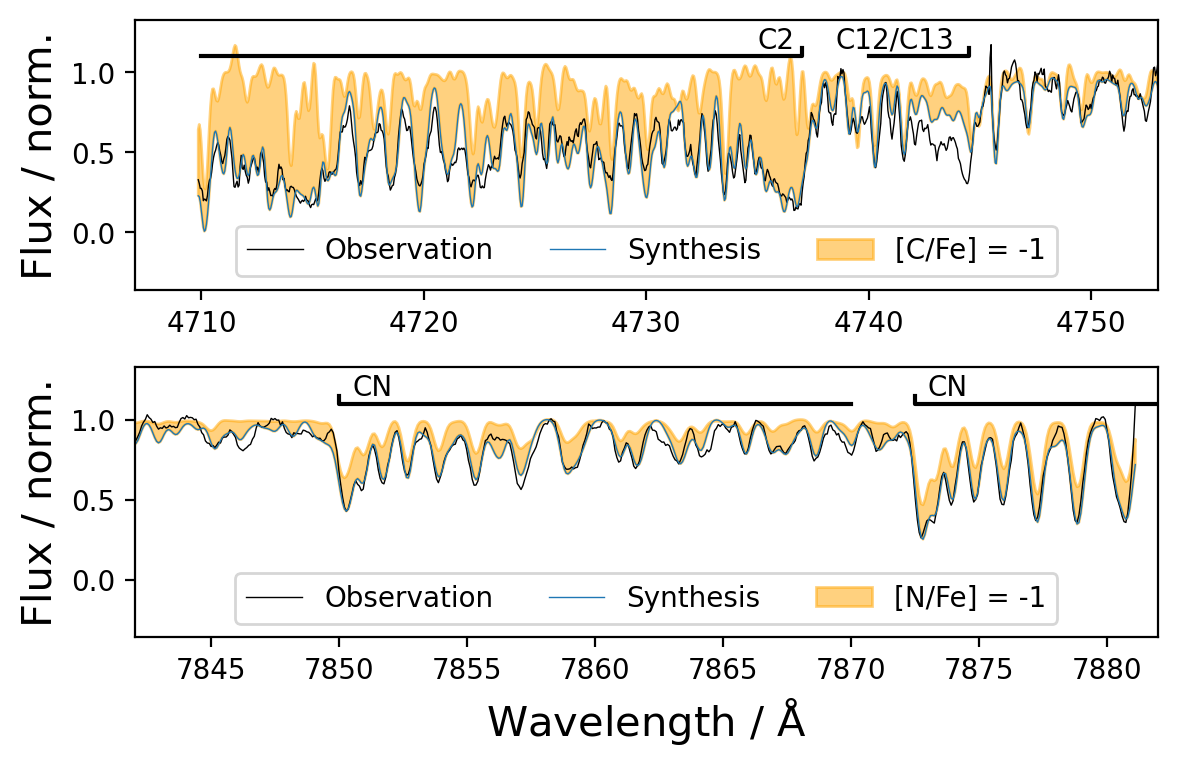
\includegraphics[width=\textwidth]{figures/c2_cn_lines_example.png}
 \caption{\textbf{Validation of C2 and CN molecular line fitting as part of GALAH DR4 for the $\mathrm{\omega Cen}$ member 2MASS J13283993-4726329.}} % 140314005201392
 \label{fig:c2_cn_lines_example}
\end{figure}



% \SB{Can we be sure, that we are interpolating properly between different models?}

% \SB{Zero points: \citet{Magg2022} for solar abundances}

%What validations do we need to include?
%
%\begin{itemize}
%    \item \Gaia FGK Benchmark stars overall \citep{Jofre2018}
%    \item Teff:
%    \begin{itemize}
%        \item ang. diameters \citep{Karovicova2018,Karovicova2020}
%        \item IRFM \citep{Casagrande2020}
%    \end{itemize}
%    \item logg:
%    \begin{itemize}
%        \item K2/Tess \citet{Zinn2020}
%    \end{itemize}
%    \item [Fe/H]
%    \begin{itemize}
%        \item intrinsic scatter in clusters: M~67, 
%    \end{itemize}
%    \item Binarity. How accurate is the flagging. Compare ratios of true/false, false-positive detections aided by \citet{Traven2020}. Get in contact with Alex Wallace and Andy Casey regarding their binarity identification from BP/RP spectra. see
%    \item Globular Clusters:
%    \begin{itemize}
%        \item \citet{Carretta2009, Carretta2009b}
%        \item NGC~104 / 47Tuc
%        \item NGC~288
%        \item NGC~362
%        \item Omega Cen: \cite{Johnson2010}
%        \item NGC~1851: \citet{Yong2015}, including CNO
%        \item NGC~6121 / M~4?
%        \item NGC~6362
%        \item NGC~6397
%        \item NGC~7099 / M~30
%        \item We have observed also NGC~4590 / M~68, NGC~5986, NGC~6144, NGC~6541, NGC~6584, NGC~6723, BH~140 and E~3.
%\end{itemize}
%    
%\end{itemize}
%
%\subsection{Caveats}
%
%\begin{itemize}
%    \item Chemical composition of \textsc{MARCS} model atmospheres do not match those of all the synthetic spectra. Ask \textsc{MARCS} people to compute them for us in next data release (as they have done for APOGEE and \Gaia)?
%\end{itemize}

\subsection{Automatic Post-Processing Performance}

In this section, we try to estimate how reliable the automatic flags of GALAH DR4 are.

Spectra have been classified by eye
% saved at GALAH_DR4/validation/spectrum_classification_by_eye.xlsx

\begin{itemize}
    \item Spectroscopic Binary Type 1 (SB1) classification, Fig.~\ref{fig:examples_flag_sp}
    \item Spectroscopic Binary Type 2 (SB2) classification, Fig.~\ref{fig:examples_flag_sp}
    \item Equivalent width estimates of three diffuse interstellar bands (5780.59, 5797.19, $6613.66\,\text{\AA}$) with central wavelengths identified by \citet{Vogrincic2023} as well as for interstellar K ($7698.9643\,\text{\AA}$), see Fig.~\ref{fig:example_dibs_06453479-0102137}
    \item Emission classification and measurement, Fig.~\ref{fig:examples_flag_sp}
    \item Upper Limit estimation
\end{itemize}

\begin{figure*}[hbt]
 \centering
 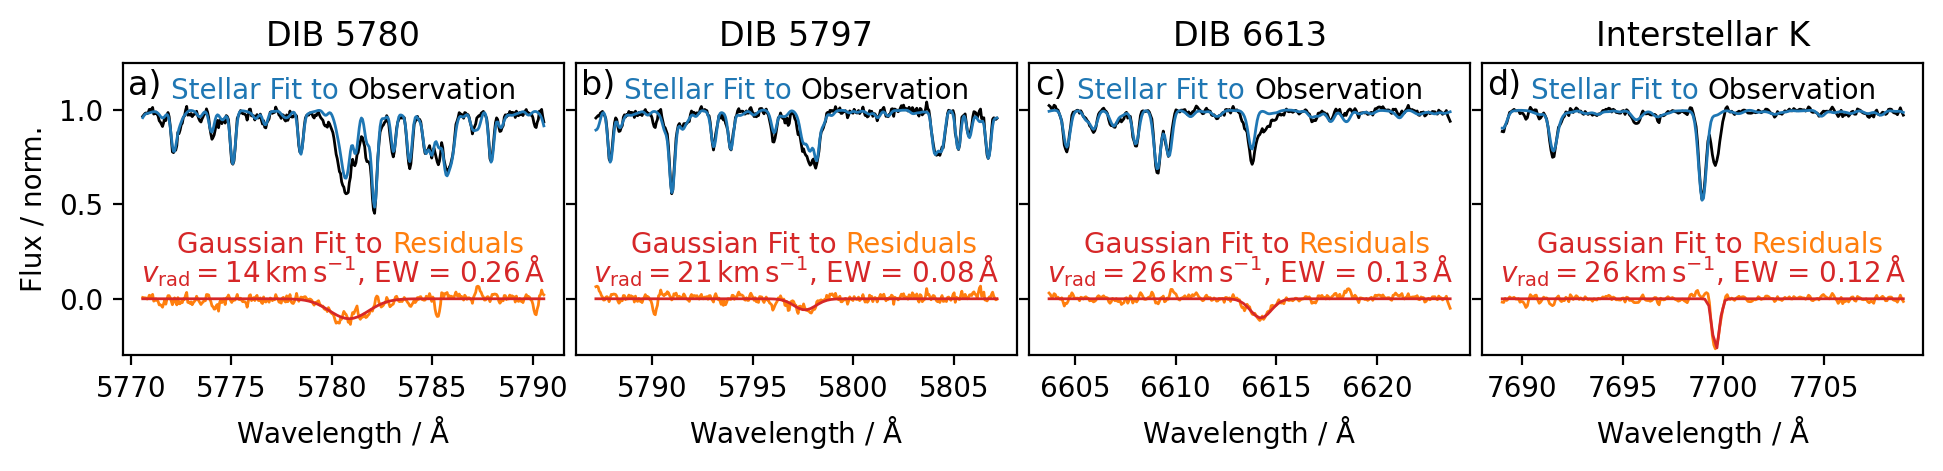
\includegraphics[width=\textwidth]{figures/example_dibs_06453479-0102137.png}
 \caption{\textbf{Example of interstellar diffuse band (DIB) and interstellar K measurements for 2MASS J06453479-0102137 with $E(B-V) = 0.84\,\mathrm{mag}$ from \citet{Schlegel1998}.}. Shown are the observation (black) and stellar fit (blue) as well as a Gaussian fit (red) to the residual (orange), resulting in an estimate of the equivalent width (EW) as well as radial velocity.} % 140314005201392
 \label{fig:example_dibs_06453479-0102137}
\end{figure*}




\newpage
%%%%%%%%%%%%%%%%%%%%%%%%%%%%%%%%%%%%%%%%%%%%%%%%%%%%%%%%%%%%%%%%%%%%%%%%%
\section{DATA RELEASE PRODUCTS}
\label{sec:catalogues_release_products}
%%%%%%%%%%%%%%%%%%%%%%%%%%%%%%%%%%%%%%%%%%%%%%%%%%%%%%%%%%%%%%%%%%%%%%%%%

\subsection{Data release catalogues}
\label{sec:data_release_catalogues}

\begin{enumerate}
   \item galah\_dr4\_allspec.fits: analysis for each spectrum (incl. RV) assuming single star
   \item galah\_dr4\_allstar.fits: analysis for each star based on co-added spectra for each star and using non-spectropic information to constrain \logg
   \item galah\_dr4\_binary.fits: analysis for those spectra that are suspected line-splitting spectroscopic binaries (SB2) assuming two sources for spectrum with same [Fe/H] but different RV
\end{enumerate}

\subsection{Data products for each spectrum}
\label{sec:data_products_for_each_spectrum}

\begin{enumerate}
   \item 210115002201239\_single\_fit\_comparison.pdf (see Fig.~\ref{fig:210115002201239_single_fit_comparison}) \SB{Maybe actually use OmegaCen star 140314005201392: cool, metal-poor, strong CNO features and a good spectrum to explain why continuum points may not always work for a pipeline.}
   \item 210115002201239\_single\_fit\_covariances.npz
   \item 210115002201239\_single\_fit\_results.fits
   \item 210115002201239\_single\_fit\_rv.png (see Fig.~\ref{fig:181221003101356_single_fit_rv})
   \item 210115002201239\_single\_fit\_spectrum.fits
\end{enumerate}

%\begin{figure*}[hbt]
% \centering  
% 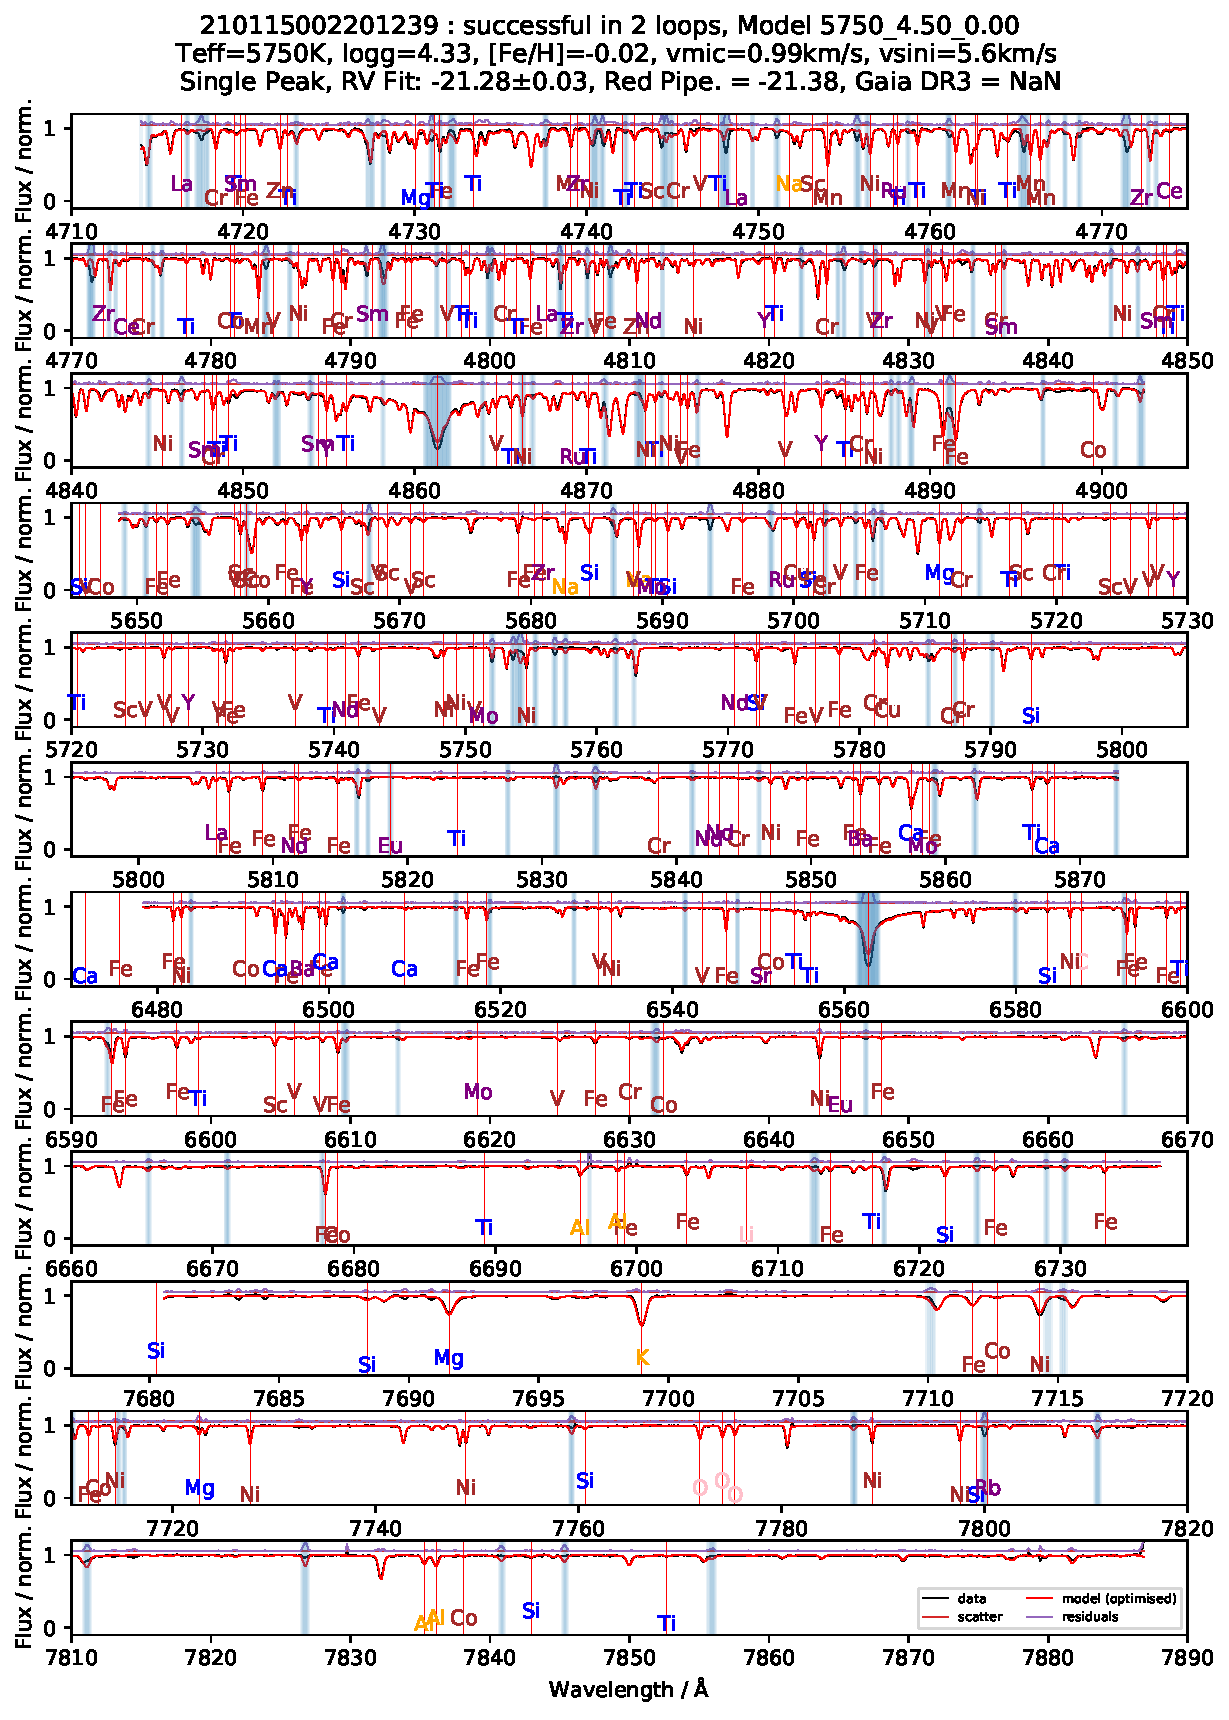
\includegraphics[width=0.9\textwidth]{figures/210115002201239_single_fit_comparison.pdf}
%\caption{\textbf{Comparison of the observed (black) and best-fit spectrum (red) for the 2dF-HERMES spectrum of the asteroid 4~Vesta.} Important element lines are annotated in each of the wavelength regions colored by their element group. Vertical areas indicate masked regions that were neglected for the label optimisation, most notably $\mathrm{H}_\beta$ at $4861\,\text{\AA}$ and $\mathrm{H}_\alpha$ at $6563\,\text{\AA}$. \SB{Maybe actually use OmegaCen star 140314005201392: cool, metal-poor, strong CNO features and a good spectrum to explain why continuum points may not always work for a pipeline. See Sec.~\ref{sec:data_products_for_each_spectrum}}} \label{fig:210115002201239_single_fit_comparison}
%\end{figure*}

\section{CAVEATS AND FUTURE IMPROVEMENTS}

\subsection{Limitations of our implemented neural networks}

While this approach has proved to be powerful for all elements across their abundance ranges, we have noticed sinusoidal shapes for weak Li lines \citep[see also][]{Wang2020}. This is likely caused by the large dynamical range that has to be covered by the neural network of $0 < \mathrm{A(Li)} < 4$. \SB{Elaborate on this! Ella's EW estimation code will limit the impact of this caveat!}

\subsection{Noding in the 3D domain}



\subsection{Unreliable wavelength solutions}

For each CCD, the reduction has found the most suitable wavelength solution, linking pixels with actual wavelengths, based on the ThXe arc lines. In GALAH DR3 \citep{Buder2021}, we have found several issues for spectra, where not enough ThXe lines could be used to constrain the wavelength solution. Improvements have been made for the new reduction version to improve the number of useful ThXe lines. Two additional pieces of information are, however, unused by the reduction pipeline, namely (i) the telluric lines that are present throughout GALAH spectra and (ii) the absorption lines of the stellar spectra. Both hold valuable information, as their position (in rest wavelength) is known very well. \SB{This has affacted mainly CCD3 with Li and Eu. One could estimate wavelength solutions from arc lines + telluric lines + absorption features.}

% The reduction is providing spectra and other parameters in an array of $n$ pixels, that is linked to wavelengths $\lambda_n$ through a linear function
% \begin{align} \label{eq:wavelength_solution}
%     \lambda (n) = \lambda_0 + n \cdot \Delta_\lambda.
% \end{align}
% In particular, for each CCD, the pipeline reports $\lambda_0$ as \texttt{cdelt} and $\Delta_\lambda$ as \texttt{CRVAl}.\footnote{\SB{Can we take into account uncertainties on these values through the pipeline? e.g. rms?}}
% Because we can directly compare to model spectra with a perfect wavelength solution, we therefore allow these eight values (two for each of the four CCDs) to be fitted by our analysis pipeline.

% \SB{Could this be degenarate with \vrad. Could be solved by (i) keeping one CCD fixed or (ii) adding a fit to the telluric lines as well, because we know their dependence on wavelength!}


\newpage
%%%%%%%%%%%%%%%%%%%%%%%%%%%%%%%%%%%%%%%%%%%%%%%%%%%%%%%%%%%%%%%%%%%%%%%%%
\section{CONCLUSIONS}
\label{sec:conclusion}
%%%%%%%%%%%%%%%%%%%%%%%%%%%%%%%%%%%%%%%%%%%%%%%%%%%%%%%%%%%%%%%%%%%%%%%%%

%%%%%%%%%%%%%%%%%%%%%%%%%%%%%%%%%%%%%%%%%%%%%%%%%%
\section*{Acknowledgements}
%%%%%%%%%%%%%%%%%%%%%%%%%%%%%%%%%%%%%%%%%%%%%%%%%%

We acknowledge the traditional owners of the land on which the AAT and ANU stand, the Gamilaraay, the Ngunnawal and Ngambri people. We pay our respects to elders past, present, and emerging and are proud to continue their tradition of surveying the night sky in the Southern hemisphere.
This work was supported by the Australian Research Council Centre of Excellence for All Sky Astrophysics in 3 Dimensions (ASTRO 3D), through project number CE170100013.

\section*{Facilities}

\textbf{AAT with 2df-HERMES at Siding Spring Observatory:}
AAT observations for this data relerase were performed under programs {2013B/13}, {2014A/25}, {2015A/3}, {2015A/19}, {2015B/1}, {2015B/19}, {2016A/22}, {2016B/10}, {2016B/12}, {2017A/14}, {2017A/18}, {2017B/16}, {2018A/18}, {2018B/15}, {2019A/1}, {2019A/15}, and {2020/B23}. This paper includes data that has been provided by AAO Data Central (datacentral.aao.gov.au).
\textbf{\Gaia: } This work has made use of data from the European Space Agency (ESA) mission \Gaia (\url{http://www.cosmos.esa.int/gaia}), processed by the \Gaia Data Processing and Analysis Consortium (DPAC, \url{http://www.cosmos.esa.int/web/gaia/dpac/consortium}). Funding for the DPAC has been provided by national institutions, in particular the institutions participating in the \Gaia Multilateral Agreement. 
\textbf{Other facilities:} This publication makes use of data products from the Two Micron All Sky Survey \citep{Skrutskie2006} and the CDS VizieR catalogue access tool \citep{Vizier2000}.

\section*{Software}

The research for this publication was coded in \textsc{python} (version 3.7.4) and included its packages
\textsc{astropy} \citep[v. 3.2.2;][]{Robitaille2013,PriceWhelan2018},
\textsc{astroquery} \citep[v. 0.4;][]{Ginsburg2019},
\textsc{corner} \citep[v. 2.0.1;][]{corner},
\textsc{galpy} \citep[version 1.6.0;][]{Bovy2015},
\textsc{IPython} \citep[v. 7.8.0;][]{ipython},
\textsc{matplotlib} \citep[v. 3.1.3;][]{matplotlib},
\textsc{NumPy} \citep[v. 1.17.2;][]{numpy},
\textsc{scipy} \citep[version 1.3.1;][]{scipy},
\textsc{sklearn} \citep[v. 0.21.3;][]{scikit-learn},
We further made use of \textsc{topcat} \citep[version 4.7;][]{Taylor2005};


\bibliography{bib}

\appendix

\section{Initial parameters}

\begin{figure*}[ht]
 \centering
 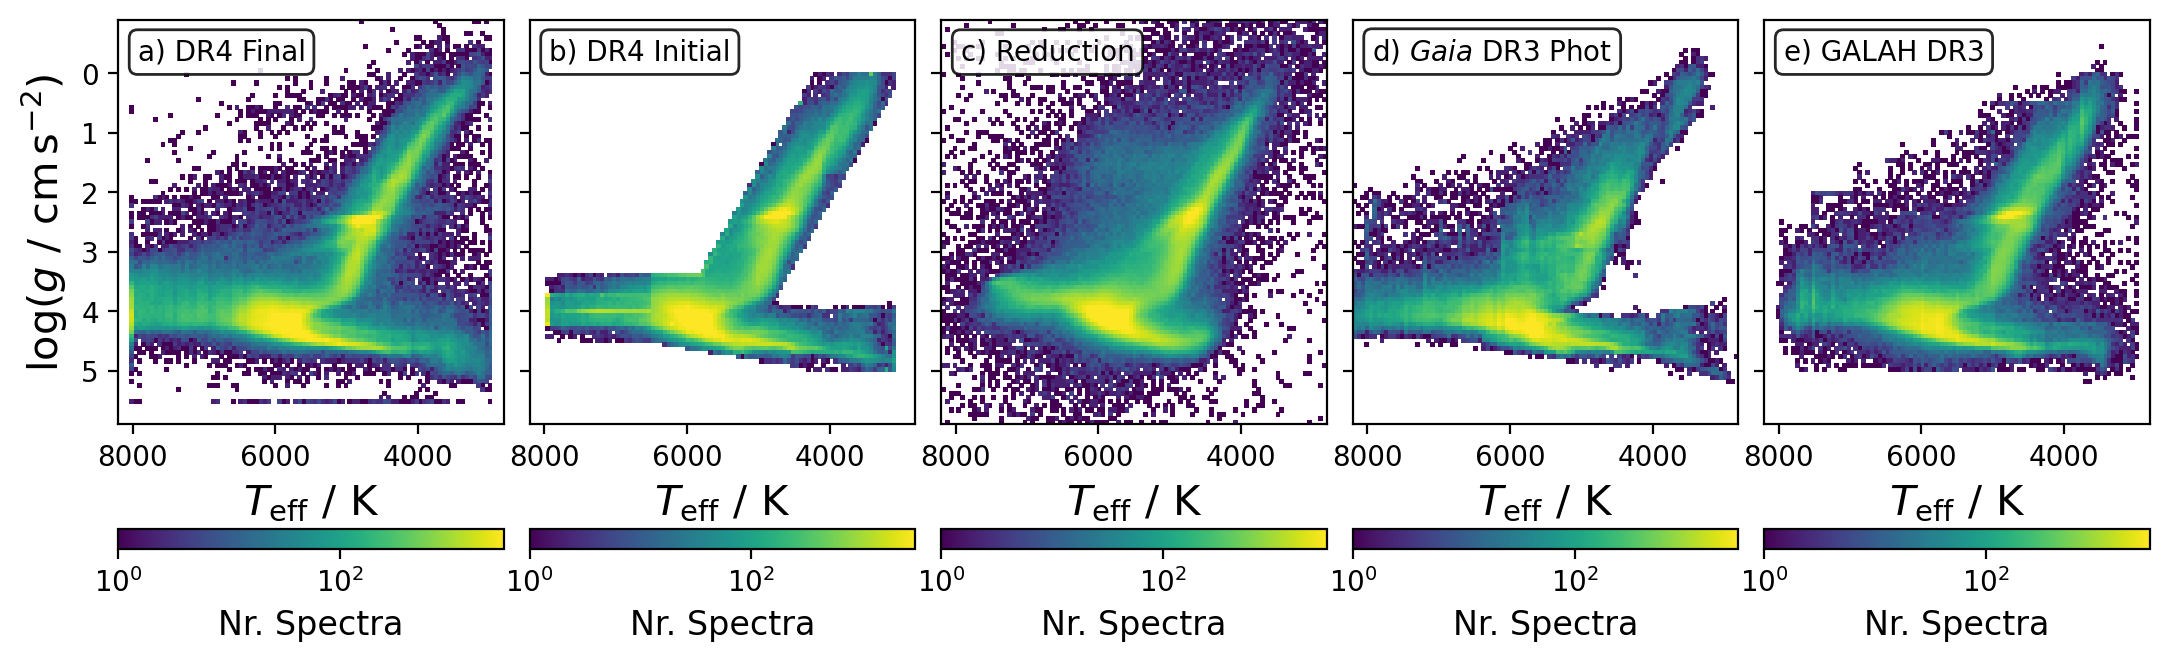
\includegraphics[width=\textwidth]{figures/initial_teff_logg.png}
 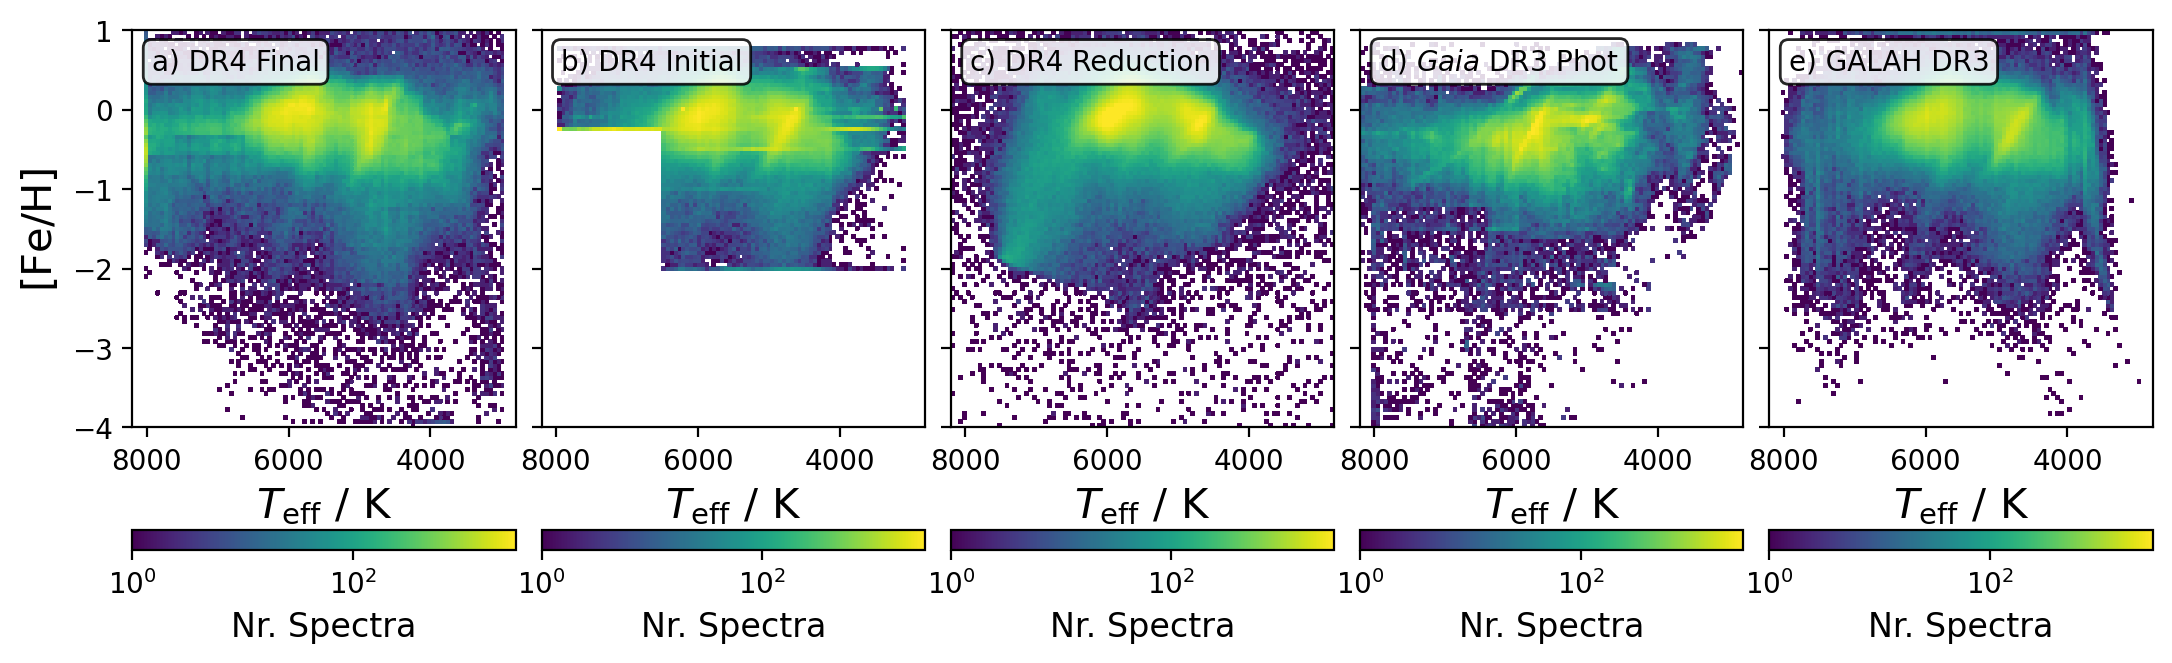
\includegraphics[width=\textwidth]{figures/initial_teff_fe_h.png}
 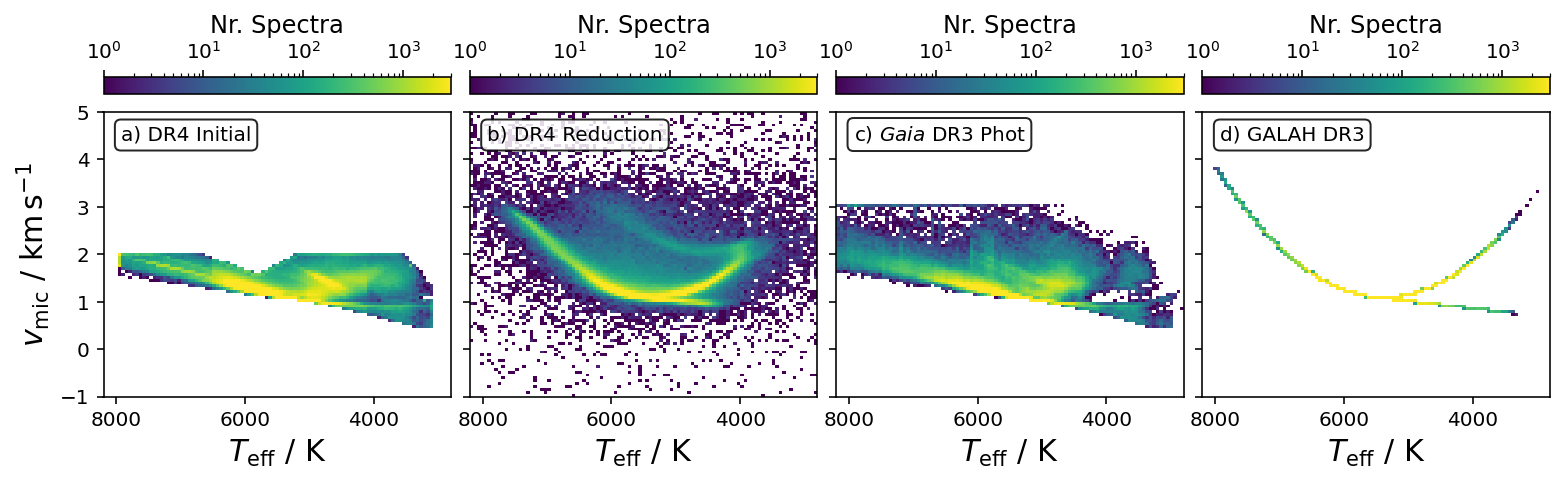
\includegraphics[width=\textwidth]{figures/initial_teff_vmic.png}
 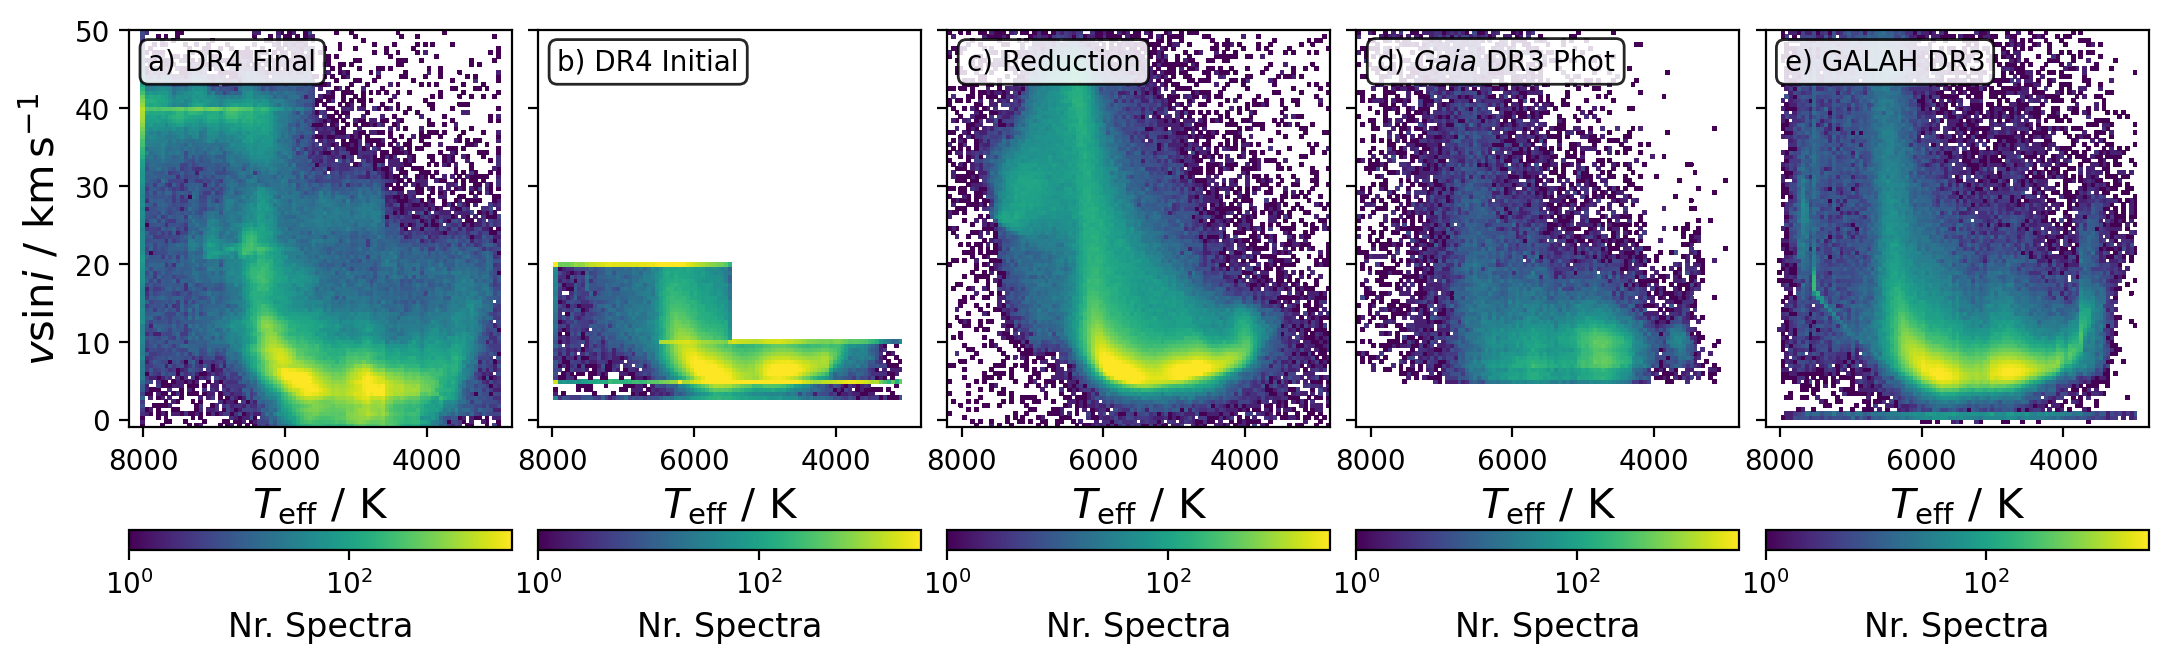
\includegraphics[width=\textwidth]{figures/initial_teff_vsini.png} \caption{\textbf{Comparison of initial parameters used for GALAH DR4 (first column) with the GALAH DR4 reduction pipeline (second column), \Gaia DR3 (third column with \vmic based on the adjusted formula from \citet{DutraFerreira2016}), and GALAH DR3 (fourth column).}} \label{fig:initial_parameters}
\end{figure*}


\end{document}
